\documentclass[]{article}

\usepackage[utf8]{inputenc}
\usepackage{array}
\usepackage{longtable}
\usepackage{graphicx}
\usepackage{multirow}
\usepackage{float}
\usepackage{caption}
\usepackage{setspace}
\usepackage{hyperref}

\title{Measuring Populism Empirically: Sentiment and Language in AMLO's Morning Conferences}
\author{Sara Cid \\  Applied Social Data Science \\  Quantitative Text Analysis}

\begin{document}

\maketitle

\begin{abstract}
	
	This study uses quantitative text analysis and dictionary methods to evaluate how Mexico's President Andrés Manuel López Obrador (AMLO) uses his morning press conferences to spread his populist message. It analyzes transcriptions from over 1300 press conferences from AMLO's start in office on December 1, 2018, to February 25, 2024. Applying a populist dictionary and performing targeted sentiment analysis on AMLO's speeches shows that he exhibits a people-centric but not so much anti-elitist language. Moreover, this paper presents novel statistics about AMLO's conferences and the evolution of his language over time\footnote{All the necessary replication files and instructions can be found under the following repository \url{https://github.com/sarabcidf/qta_amlo_24}}.

\end{abstract}

\section{Introduction} 

In the past decades, the rise of populism across the world has sparked interest among scholars, leading to research about its defining characteristics and the strategies employed by populist leaders. Central to the research on populism are the questions of whether populist leaders are inherently anti-elite and people-centric to resonate more with the common people. This study aims to contribute to this ongoing debate by examining the rhetorical strategies of Andrés Manuel López Obrador (AMLO), the President of Mexico, known for his distinctive and populist approach to political communication. Transcriptions of AMLO's \textit{mañaneras} or daily morning press conferences provide the corpus for the present analysis. During these conferences, AMLO engages with the media and with the public directly, speaking about current issues and policy, and answering questions. By analyzing over 1300 transcripts of these conferences, which span from his inauguration on December 1, 2018, to February 25, 2024, this study analyzes AMLO's rhetoric in search for populist traits.  

The broader research question that guides this study can be phrased as follows: \textit{Are the tendencies to oppose the elite and advocate for the common people characteristics of populist rhetoric?} and, more particularly, \textit{Are these tendencies present in AMLO's discourse?} Thus, this study seeks to determine whether AMLO's speech is predominantly anti-elite and people-centric, characteristics commonly attributed to populist leaders. By addressing this question, this study sheds light on AMLO's communicative style, and it contributes to a deeper understanding of populism as a political phenomenon and as a communication style or strategy. Using a populist dictionary and targeted sentiment analysis, this study provides empirical evidence on the extent to which these traits are present in AMLO's language. 

In addition, an assessment of speech readability and lexical diversity was attempted, but there is reason to believe its results are unreliable, especially in the case of readability. Unfortunately, the computation of a measure of readability adequate for the Spanish language was beyond the reach of this study, and the more readily available tools for English are not reliable in this case. The results are nonetheless presented in the Appendix, along with a more detailed discussion of the validity and reliability of the measures that were used, in case this is of relevance for future research. 

\section{Literature}

The political science and communication literature contains numerous articles on populism and language. Firstly, papers like that of de Vrees et al., \cite{de_vreese_populism_2018} link populism with a particular language, rhetoric and communication style, suggesting that the latter are defining features of the former. Given that populist language has been advanced as characteristic of populist leaders, some researchers have thus gone on to study this language. Among these studies, some, like (\cite{decadri_populism_2020}) , or \cite{rooduijn_measuring_2011}, have used computer-assisted quantitative text analysis to measure populism through language, finding that populist ideology, electoral strategy, and party membership lead to the use of a particular and simpler language in communication. 

Moreover, some articles have focused on particular leaders. Kreis' \cite{kreis_tweet_2017} examination of President Trump's use of Twitter as a strategic communication tool to propagate right-wing populist discourse shows the importance of social media in modern populist rhetoric, and Lamont et al.'s \cite{lamont_trumps_2017} analysis of Trump's electoral speeches further illustrates how populist leaders articulate the grievances of marginalized groups, positioning them against perceived elite oppressors and external threats.

As Decadri \& Boussalis point out, \cite{decadri_populism_2020}, however, comprehensive empirical studies on populist communication style are still quite rare. By shedding light into how AMLO's language distinguishes between the people and the elite, the present paper would thus add to this literature, while also helping to close the gap in knowledge about these phenomena in the developing countries, as this is currently lacking (Hawkins' \cite{hawkins_is_2009} study on Hugo Chávez and other Latin American leaders is one of the few academics that have applied a quantitative methodology to study populist leaders outside the developed world.). 

\section{Context: Andrés ManueL López Obrador and the Morning Press Conferences}

Andrés Manuel López Obrador (AMLO), Mexico's current president, is a figure of great interest in the landscape of Latin American politics and populism studies. By the time he ascended to the presidency, AMLO had a long and distinguished political career. He acted as the Mayor of Mexico City from 2000 to 2005, where he gained immense popularity. After experiencing setbacks when running for president in the 2006 and 2012 elections, AMLO established his own political party, the National Regeneration Movement (MORENA), in 2014 \cite{navarrete_vela_morena_2019}. This movement, along with considerable discontent of the Mexican electorate with the ruling parties, catapulted AMLO to the presidency with a landslide election in 2018 \cite{moreno_viraje_nodate}. 

AMLO's \textit{mañaneras}, his morning press conferences, have become distinctive of his presidency, as they are a new approach to political communication in Mexico. These sessions, beginning at 7 a.m. almost every day, typically last between one and two hours, and are broadcasted live on various media platforms. Through them, AMLO addresses a wide array of topics, from policy announcements and government achievements to responses to criticism and current events. By some estimates, an average of 10M people watch or listen to AMLO's conferences every day \cite{bravo_5_2024}. Also, the descriptive analysis for this paper revealed that the word count of the conferences has increased over time, although their monthly frequency has decreased (see the Appendix). 

For AMLO's supporters, the conferences are an act of transparency, access to information, and freedom of expression, as they offer journalists the opportunity to directly ask the president about public affairs. For critics, these conferences are a toxic and polarizing abuse of presidential power and have nothing to do with transparency or information, as AMLO often does not answer, evades, or gets upset by questions. According to this view, AMLO uses these conferences for communication, propaganda and to attack the media and other institutions that oppose him, such as the Supreme Court of Justice or the National Electoral Institute. The conferences have been criticized by major international organizations such as the European Parliament, the Inter-American Court of Human Rights, and the International Press Institute \cite{najar_asi_2019}. According to various experts, the conferences serve as a direct channel for AMLO to communicate with the Mexican citizenry, bypassing traditional media outlets that he often criticizes for their alleged bias. As such, the conferences grant AMLO great agenda-setting and disseminating power, as he is able to control public discourse through them \cite{zapata_mananeras_2022}.

\section{Methodology}

Over 1300 press conference transcripts were gathered, cleaned and processed into a Document-Feature-Matrix (DFM) for the quantitative analysis of the text. All of the transcripts available in AMLO's website \cite{noauthor_transcripciones_nodate} were scraped, then these were filtered by title to keep only those belonging to morning press conferences (as this website also contains transcripts from extraordinary conferences, events and speeches), and then the text was filtered to keep AMLO's words only (eliminating any interventions by members of his cabinet, the press or any other participants). From this, a corpus was created. This corpus was later tokenized, cleaned and converted into the DFM for study. 

The analysis of AMLO's rhetoric followed two main strategies. First, Spanish versions of the AFINN and NRC sentiment analysis dictionaries were applied to AMLO's rhetoric. These dictionaries were translated by Data Scientist Juan Bosco \cite{vega_lexicos_2023}, and simplified to be binary (words are either positive or negative in sentiment, rather than assigning scores). Figure 1 below shows that the application of both dictionaries should be consistent, as there is significant overlap between the net sentiment that both produce, with AFINN detecting slightly more negative sentiment in AMLO's language.

\begin{figure}[H]
	\centering
	\caption{\label{}}
	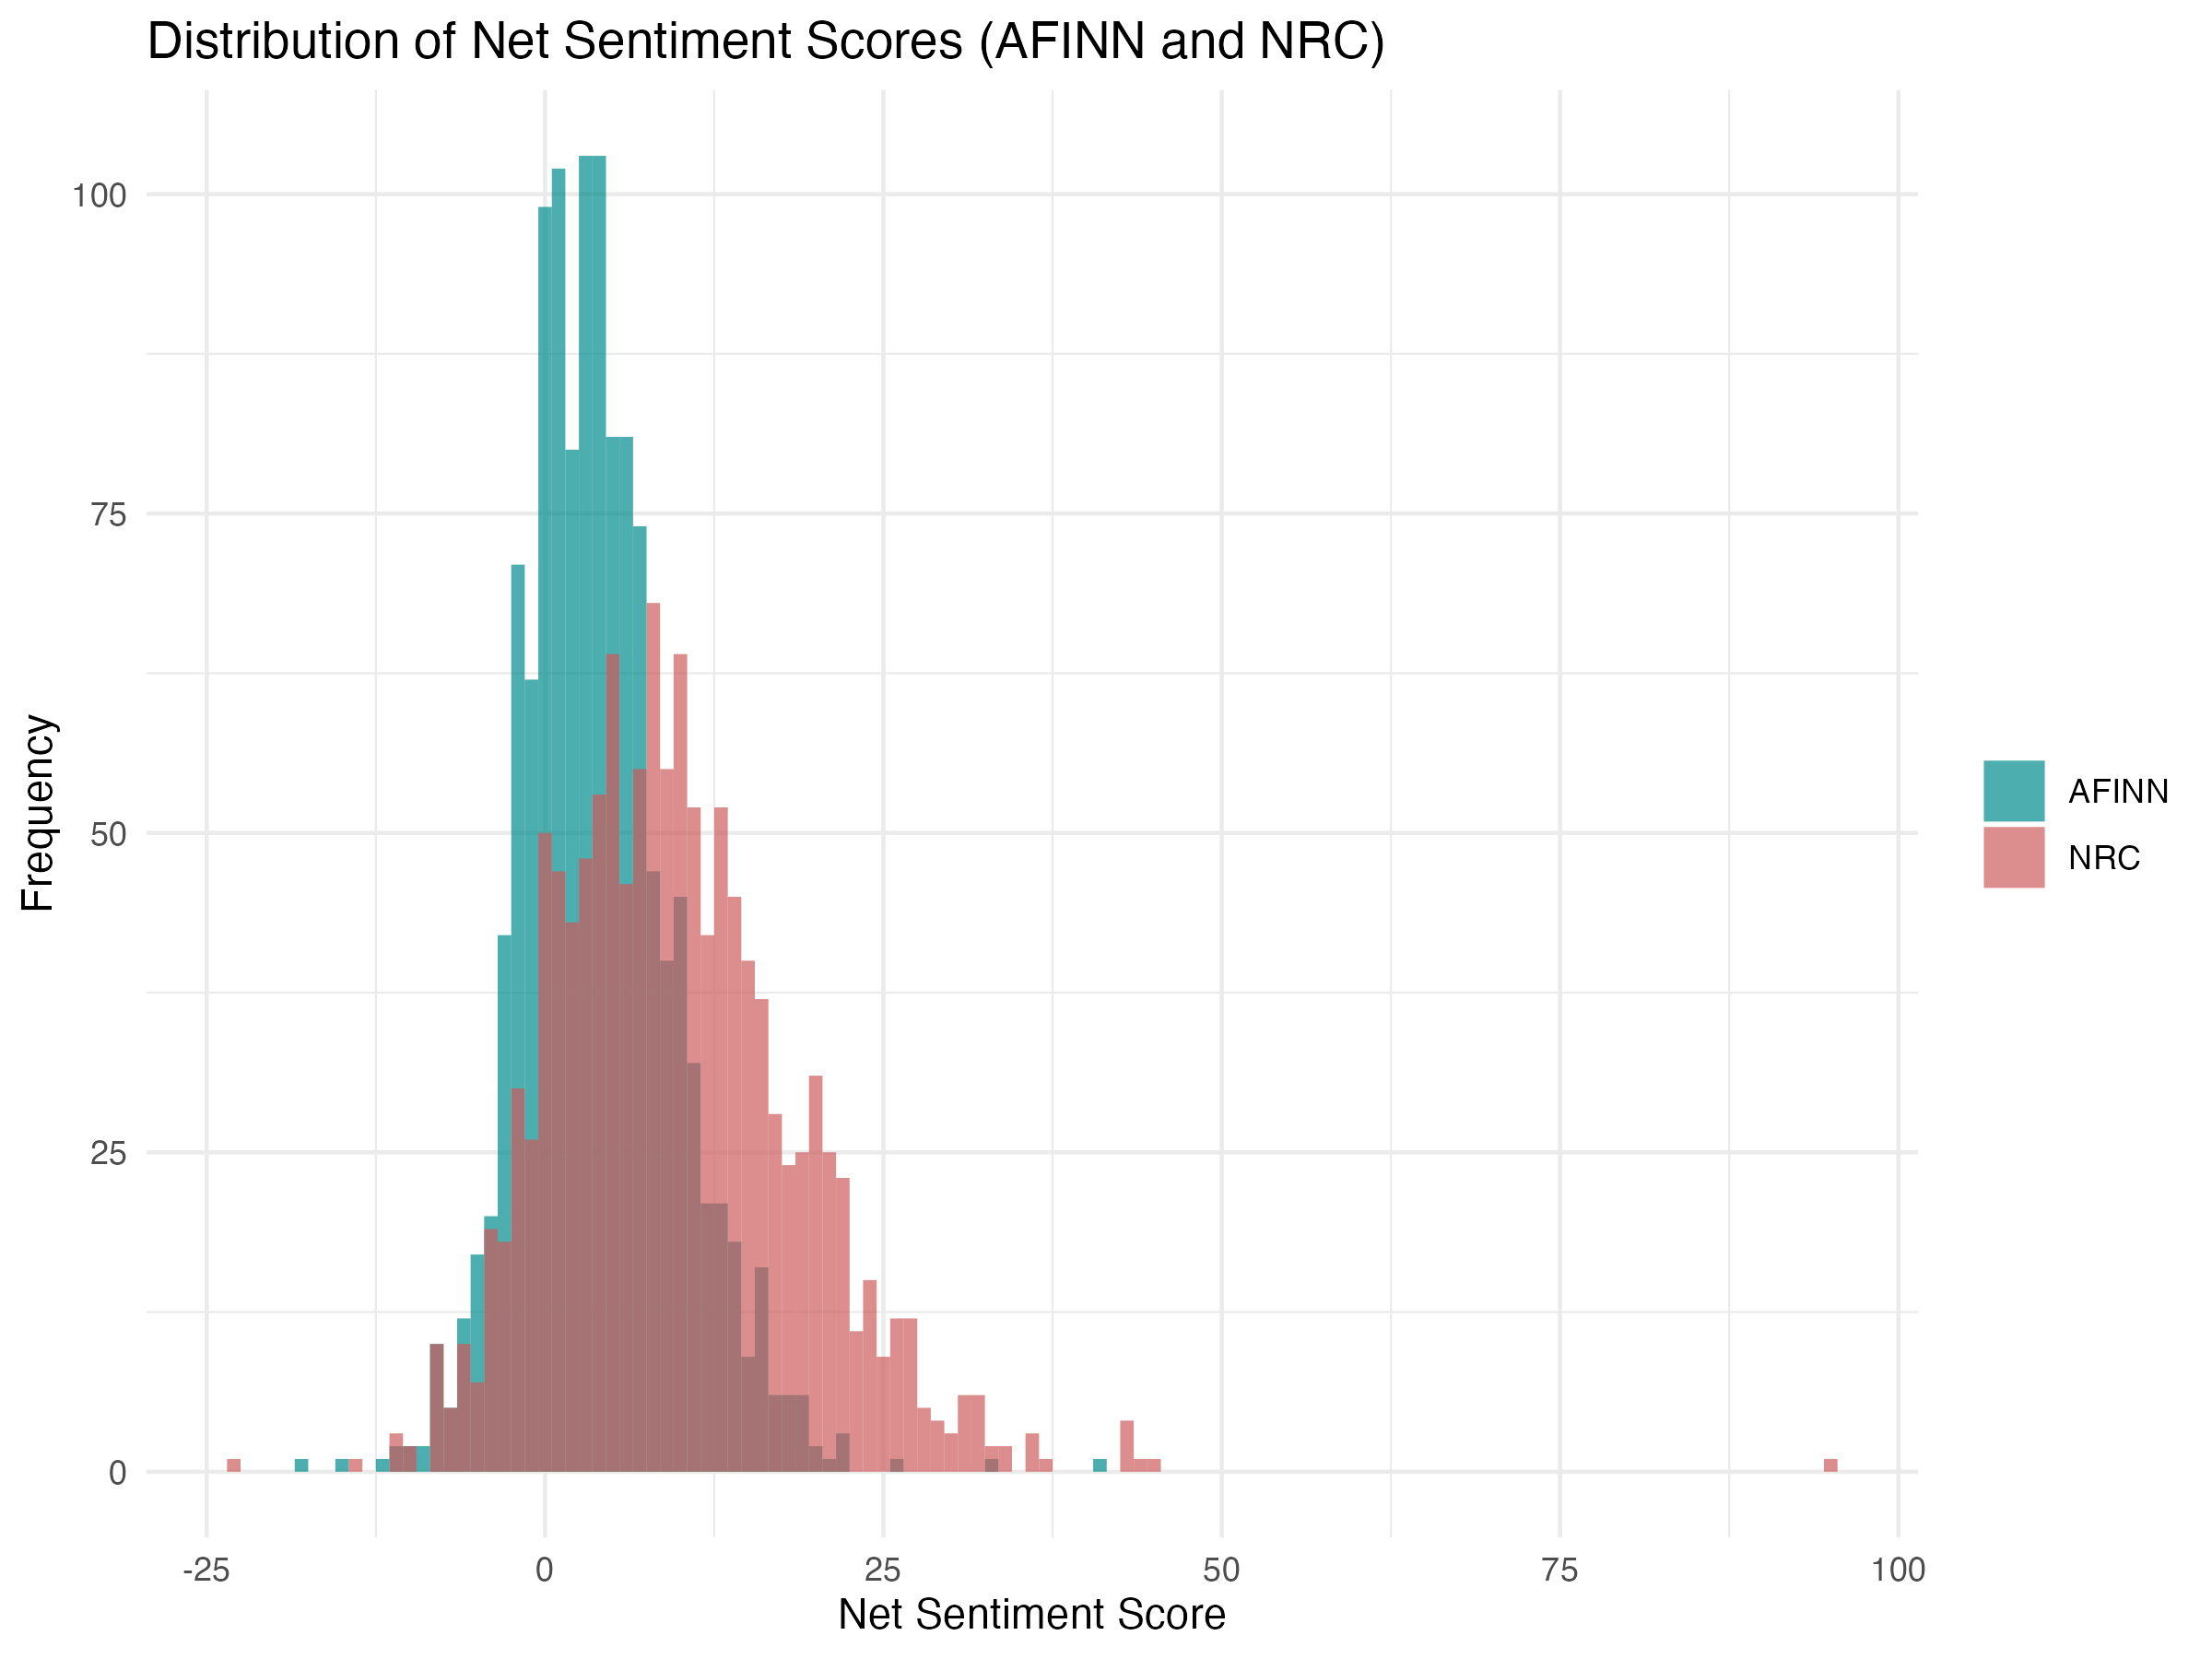
\includegraphics[width=\textwidth]{/Users/sarabcidf/Desktop/ASDS/Dissertation/AMLO/Analysis/sentdistrib.png}
\end{figure}

Second, another dictionary method was used to evaluate AMLO against a list of populist terms. This list was originally developed by \cite{rooduijn_measuring_2011}, and then expanded by Decadri \& Bousalis \cite{decadri_populism_2020}. The analysis was conducted against both the original and the expanded version, and against two further expansions that were developed for this study, considering the Mexican context. To ensure consistency and reliability in this second method, no one version of the populist dictionary was applied on its own, but rather the four versions (resulting of both originals and their expansion) were applied, and the results across all applications were similar, showing consistency. This is shown in the Results section below, and the dictionaries can be consulted in the Appendix. 

The entirety of the analysis was carried out in R, with the help of Quanteda \cite{quanteda2018} and other packages. Additionally, an analysis of readability and lexical diversity was attempted. This would serve to test whether the populist trait of speaking in a simple manner that is appealing to the average citizen applies to AMLO. However, as it is explained in the Introduction, reliability is a major concern here. The results and a discussion are nonetheless presented in the Appendix. 

\section{Results}

\vspace{.5cm}
\noindent\textbf{Targeted Sentiment Analysis}
\vspace{.5cm}

\noindent 

More statistics about the general sentiment of AMLO's speech can be found in the Appendix. This section concentrates on the analysis targeting keywords. The two following figures show the results of such targeting, first using the AFINN dictionary, and then the NRC. Following the hypotheses, this exercise should show that AMLO exhibits negative sentiments around elites
\footnote{The keywords to evaluate sentiments around elites and the establishment were the Spanish translations of conservative(s), "mafia", "elite(s)", "mafia in power", "Prian" (used by AMLO to refer to the PRI and PAN parties) and "conservative block"} 
and positive sentiments around the people
\footnote{The keyword to evaluate sentiments around the people was the Spanish translation of people.}. 
In addition, the hypotheses that AMLO exhibits positive sentiments towards his infrastructure projects
\footnote{The keywords to evaluate sentiments around these projects were the names of these, namely "Felipe Ángeles", after AMLO's airport, "Guardia Nacional", after AMLO's national guard, "Dos Bocas" and the Spanish translation of oil refinery, for his refinery mega-project, and "Tren Maya", for the touristic train, another of his mega-projects} 
and his social programs
\footnote{Here, as well as with the projects, the keywords were the names of the programs, namely Sembrando Vidas, Adultos Mayores and Jóvenes Construyendo el Futuro}, 
while exhibitting negative sentiments towards contrary institutions
\footnote{The keywords to evaluate sentiments around institutions that AMLO seems to perceive as contrary to him were the name of the Electoral Institue of Mexico and its acronym, the same for the Central Bank, and the same for the Supreme Court, as well as the Spanish word for judges.} 
and the media
\footnote{Finally, the keywords used to measure sentiment around the media were the names of some of the largest newspapers in Mexico, the Spanish words for media and newspaper, and the names of some of the top Mexican journalists (Aristegui, López Dóriga, Ciro Gómez Leyva, Loret de Mola, etc.)}. 

\begin{figure}[H]
	\centering
	\caption{\label{}}
	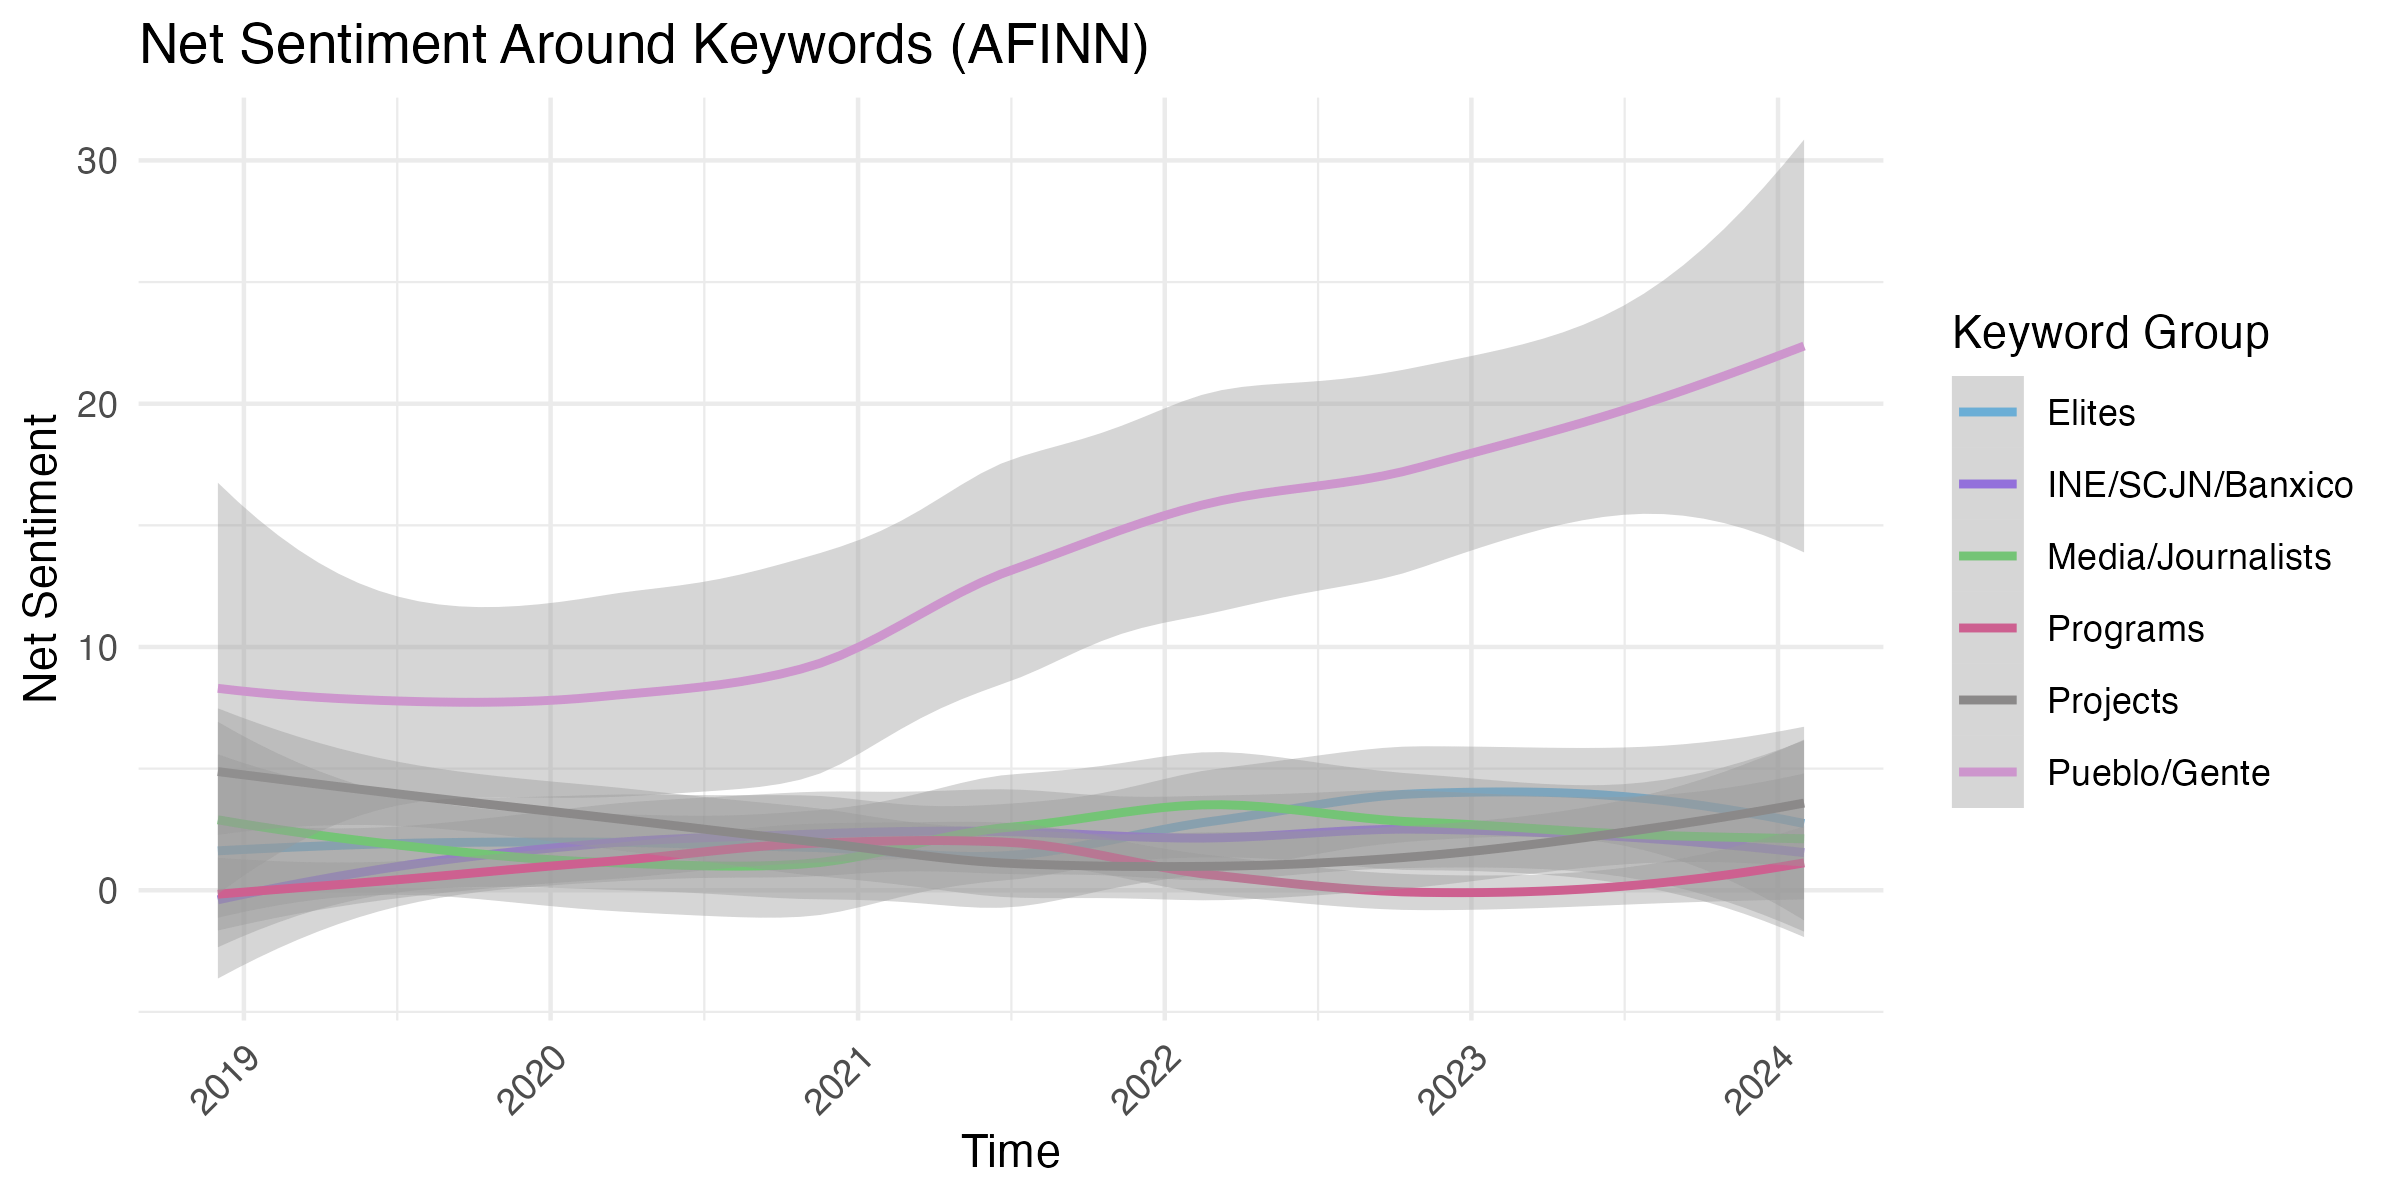
\includegraphics[width=\textwidth]{/Users/sarabcidf/Desktop/ASDS/Dissertation/AMLO/Analysis/targsaafinn.png}
\end{figure}

\begin{figure}[H]
	\centering
	\caption{\label{}}
	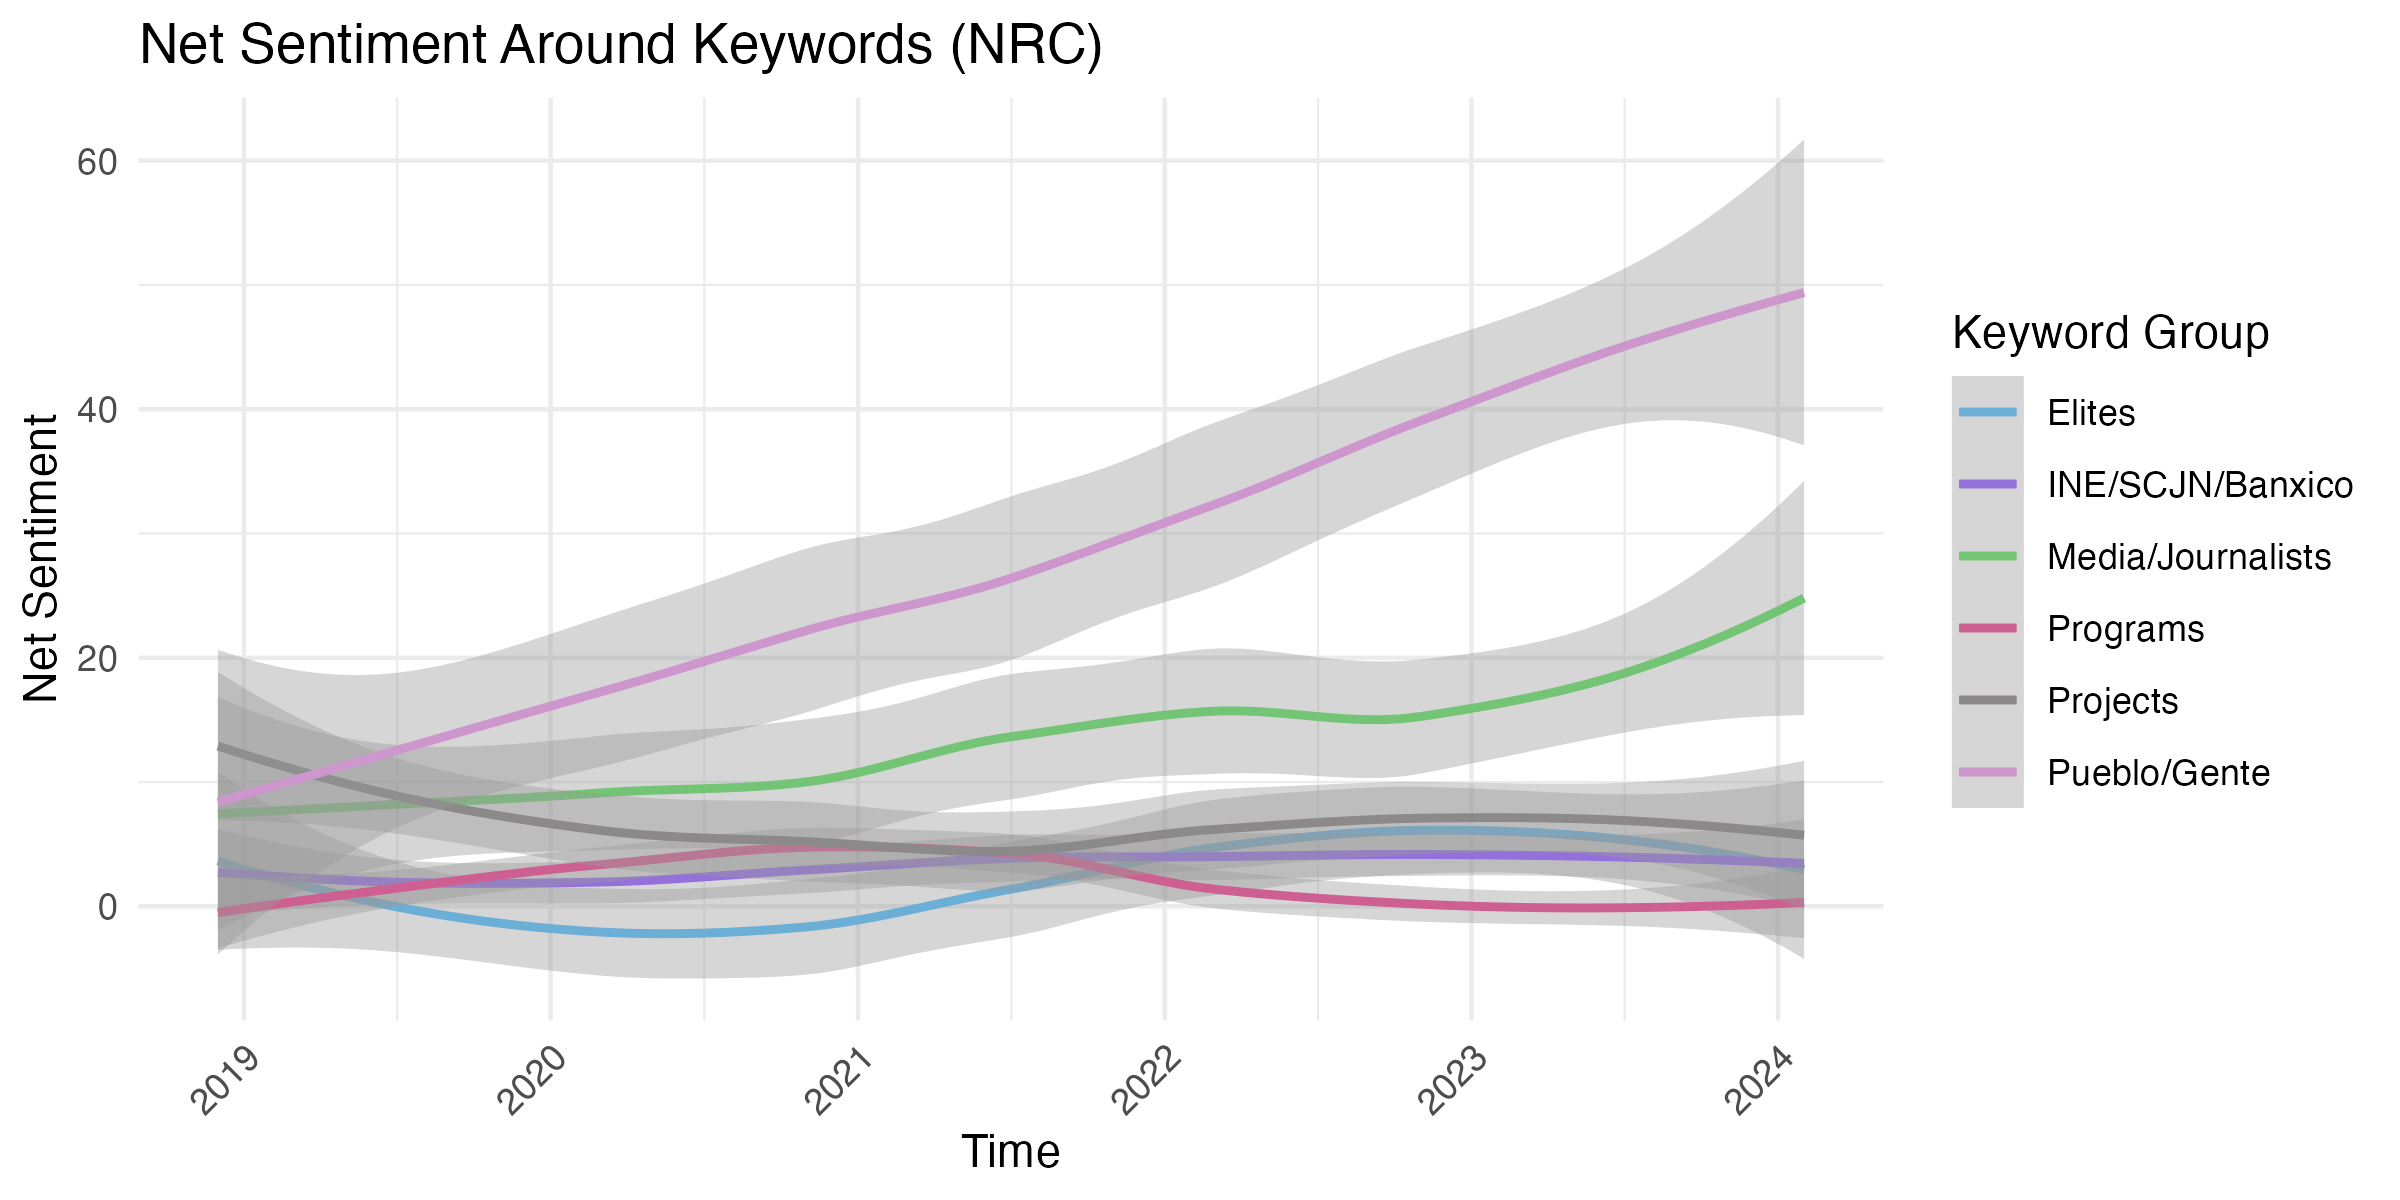
\includegraphics[width=\textwidth]{/Users/sarabcidf/Desktop/ASDS/Dissertation/AMLO/Analysis/targsanrc.png}
\end{figure}

While the results show evidence in favor of the positive sentiment around the people, AMLO's sentiment around other keywords and groups of keywods is less consistent. According to the plot resulting from AFINN, the sentiment around keywords referring to AMLO's projects and programs is, at times, lower than that around opposing institutions/elites. The results for sentiment around people are consistent in the NRC graph as well, while this second graph suggests AMLO's sentiments around the media have improved over time. Overall, the analysis suggests that AMLO feels extremely positive around the people, while he does not really express negative sentiment around institutions or the media, nor does he display positive sentiment around his projects or programs.

\vspace{.5cm}
\noindent\textbf{Application of Populist Dictionary}
\vspace{.5cm}

\noindent Finally, AMLO's rhetoric was evaluated against a dictionary of populist terms. Several versions of the dictionary were used: firstly, the original version of the populist dictionary, developed by Rooduijn \& Pauwels \cite{rooduijn_measuring_2011}, which is formed by typical anti-elitist words. This is the "original anti-elitism" dictionary shown in the next Figure. "Second, an extended version of this dictionary, with additional anti-elitist terms particular to the Latin American and/or Mexican context was applied. This is the "expanded anti-elitism" dictionary in the Figure below. The third dictionary that was applied was that developed by Boussalis \& Decadri \cite{decadri_populism_2020}, who expanded on the original anti-elitist dictionary, adding people centrist-terms. This third dictionary is named "original people-centrism" Finally, a fourth version of the dictionary where further Mexico-specific people-centrism terms were added was also applied. This is the "extended people-centrism" below. A more detailed discussion on how the dictionaries were extended with context-specific terms is provided in the Appendix. 

As Figure 4 below shows, both versions of the people-centrism dictionary apply better than both versions of the anti-elitism ones to AMLO's speech. This is consistent with the results from the targeted sentiment analysis. In addition, the figure shows an upward trend in the usage of populist vocabulary overtime. From the targeted sentiment analysis, it would be reasonable to assume that the word driving this trend is "people". However, there is also a slight trend upward in anti-elitism vocabulary usage, and for the extended version of this dictionary we observe a peak around the middle of 2023, which could reflect AMLO's response to criticism surrounding his interventions regarding the State of Mexico's governor election. 

\begin{figure}[H]
	\centering
	\caption{\label{}}
	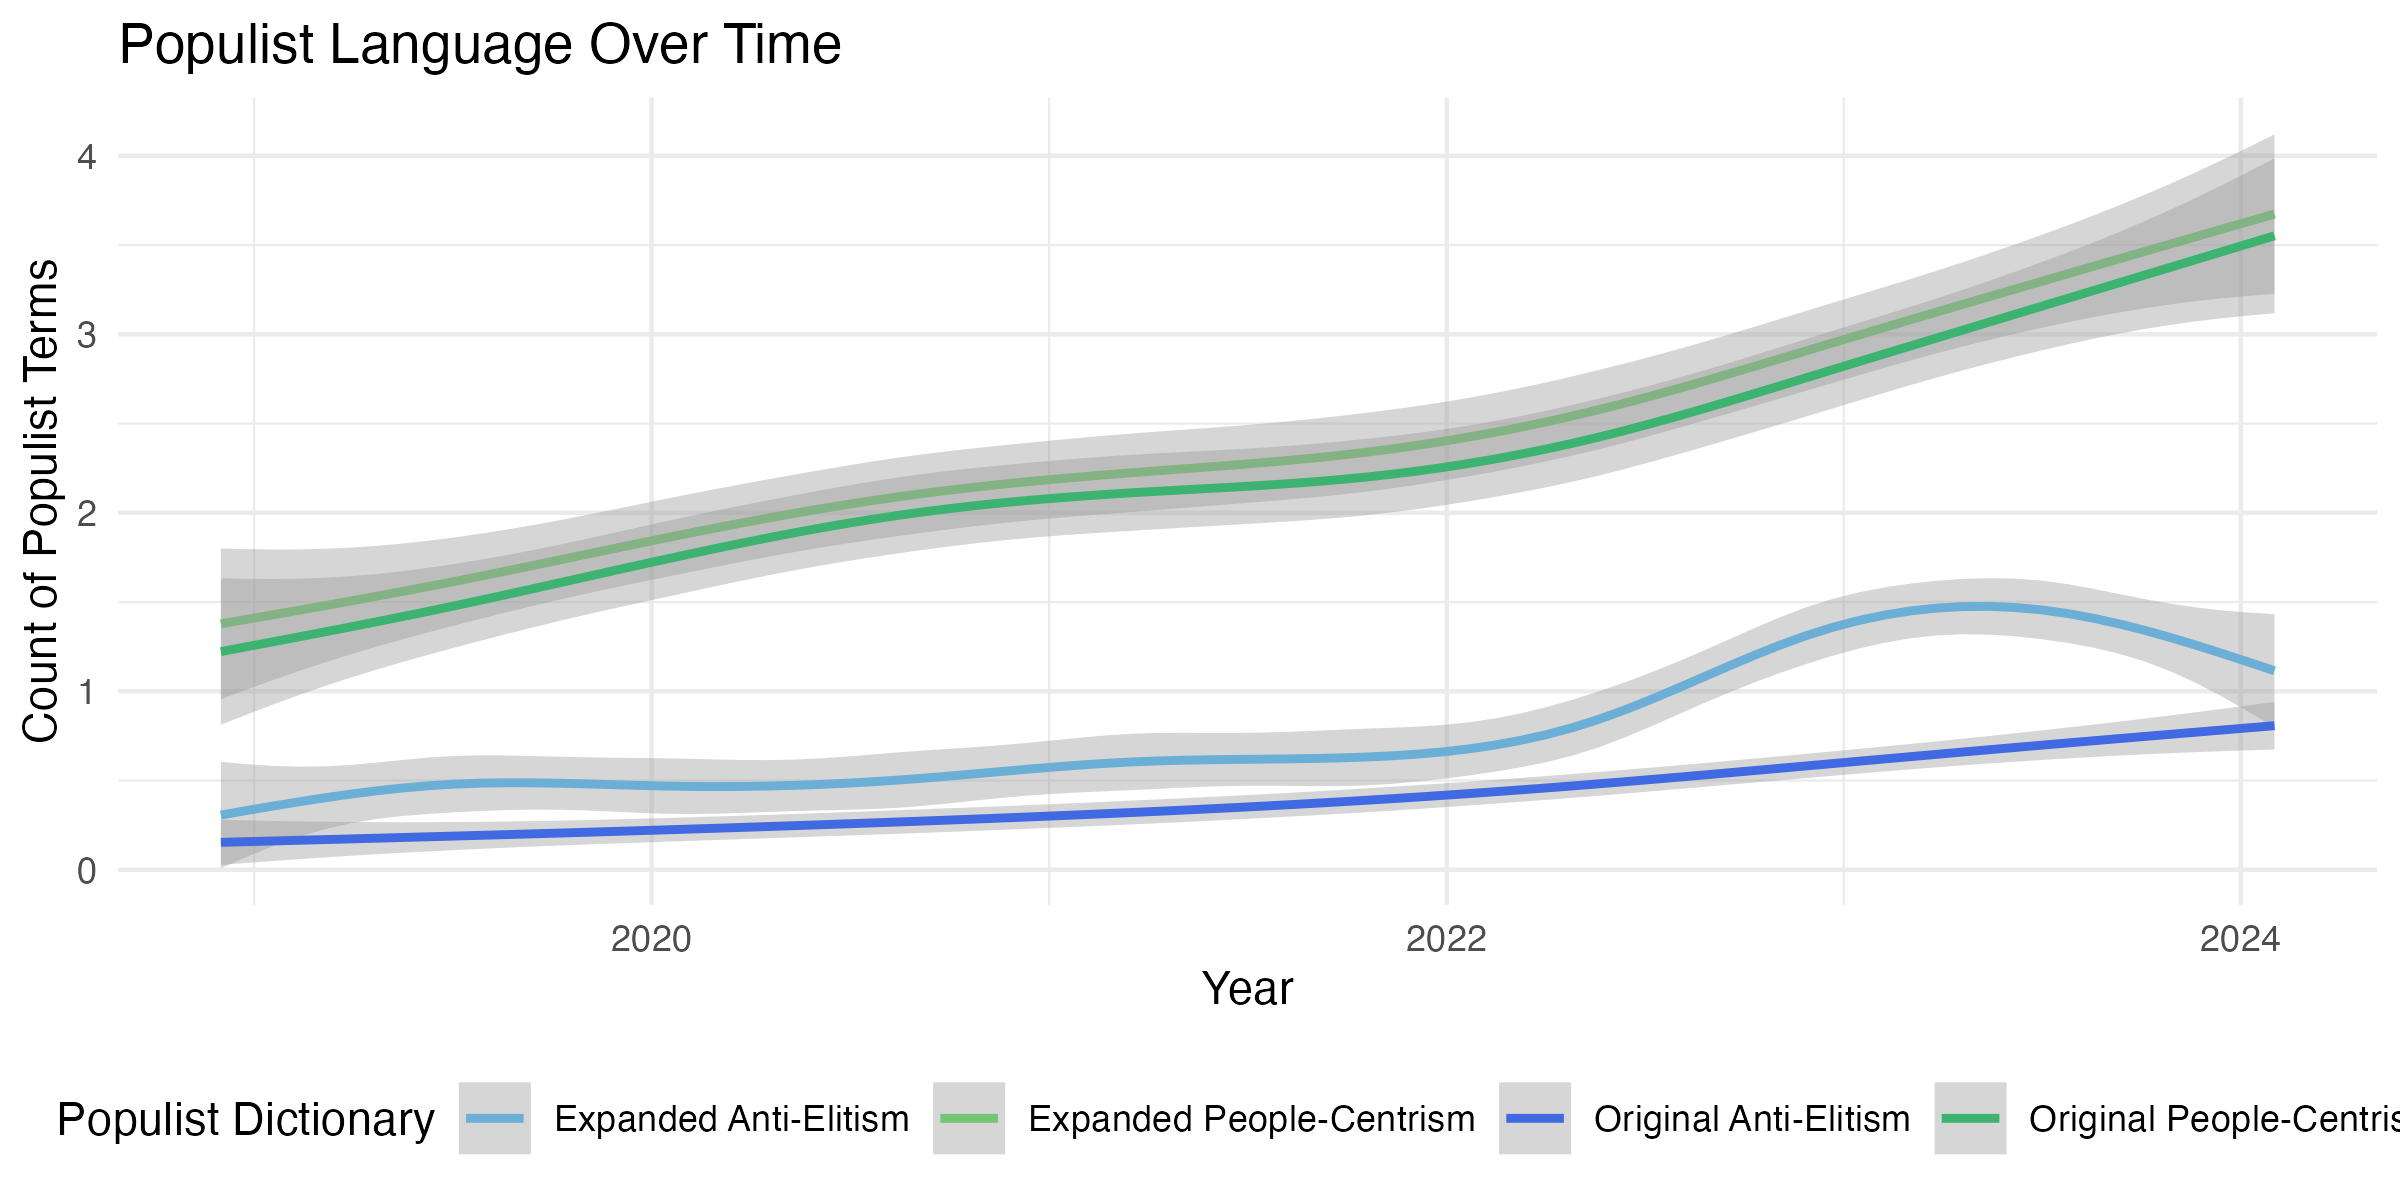
\includegraphics[width=\textwidth]{/Users/sarabcidf/Desktop/ASDS/Dissertation/AMLO/Analysis/poplangtimecount.png}
\end{figure}

\section{Conclusions}

This study investigated how AMLO, the President of Mexico, addresses the media and the public in his morning press conferences. The main finding is that AMLO often talks positively about ordinary people, fitting with the populist people-centric language thesis. This positive sentiment around the people has become more pronounced overtime. While there is also some evidence of anti-elitist vocabulary in AMLO's language, his comments on government institutions, the media, and his policies do not seem to clearly follow the expected populist attack on elites/adversaries or praise/propaganda for his initiatives. Through this analysis, the present paper has added to our understanding of populism, populist language, and its characteristics by showing that AMLO's communication style is complex and beyond just being anti-elite or solely pro-people. 

\section{References}

\bibliographystyle{plain}
\bibliography{PopulismBib}

\vspace{.5cm}
\section{Appendix}

\vspace{.5cm}
\noindent\textbf{Summary Statistics}
\vspace{.5cm}

As shown in Figures 5, 6, and 7 below, both the length of the press conferences (measured by the number of words) and the its variation seem to increase overtime, while the frequency of AMLO's press conferences has decreased slightly. Additionally, Figure 8 reveals that some interesting words are among the most frequent in the conferences corpus. Words surrounding information are frequent, as are the two different Spanish words for "people". This last element suggests that AMLO does not just have a people-centric language, or speaks favorably about the people, he also speaks a lot about the people. The word corruption is also among the most frequent, which is consistent, as battling corruption is one of AMLO's main promises.  

\newpage
\vspace*{\fill}

\begin{figure}[H]
	\centering
	\caption{\label{}}
	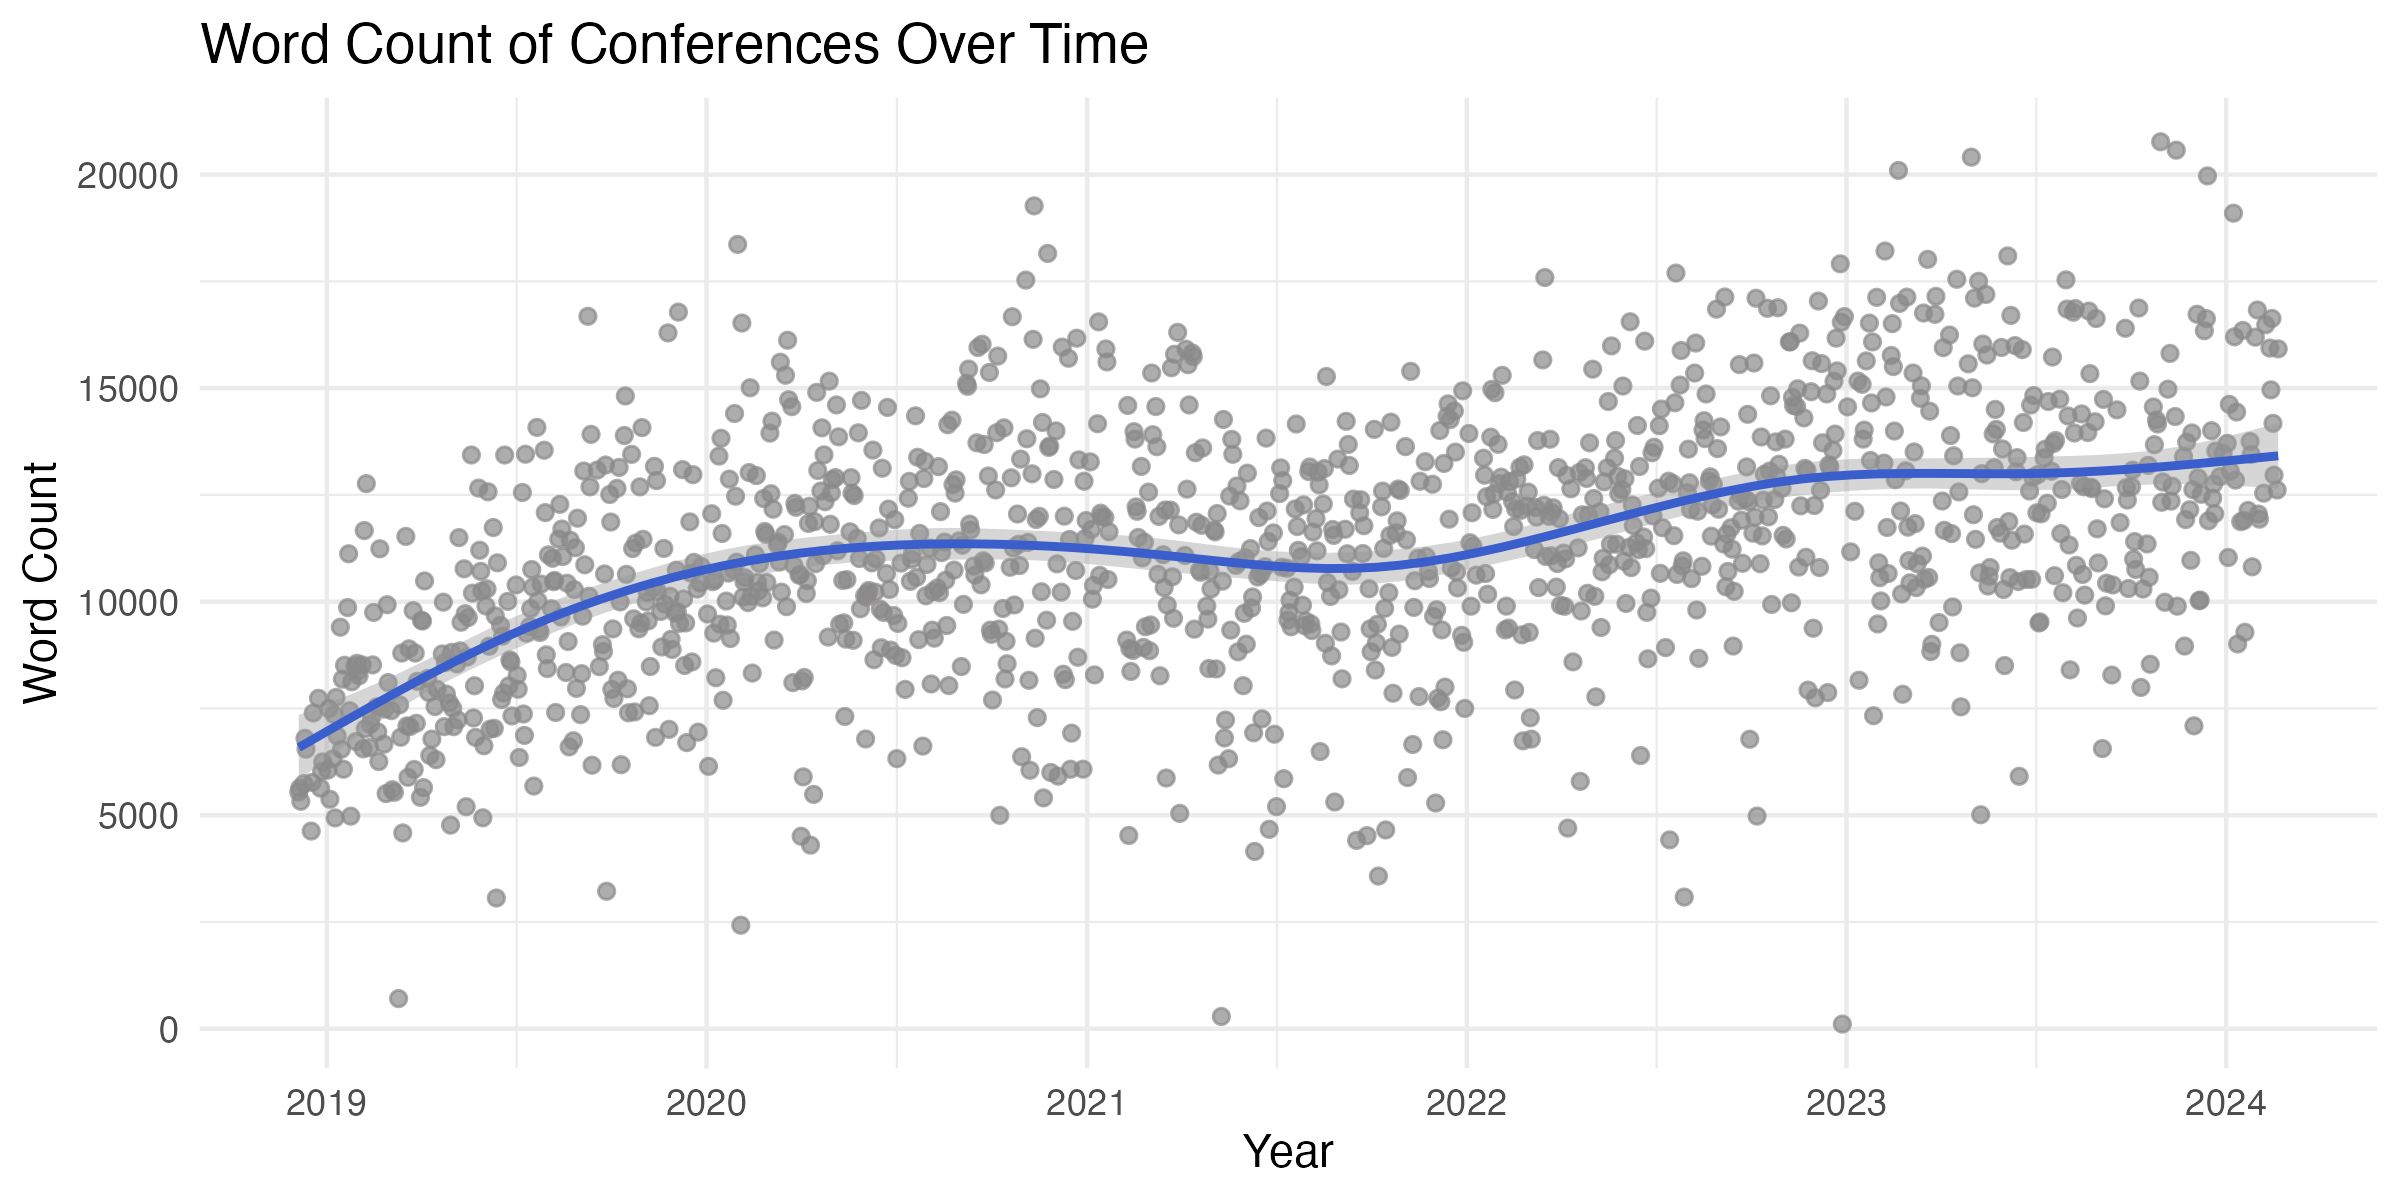
\includegraphics[width=\textwidth]{/Users/sarabcidf/Desktop/ASDS/Dissertation/AMLO/Analysis/words_time.png}
\end{figure}

\begin{figure}[H]
	\centering
	\caption{\label{}}
	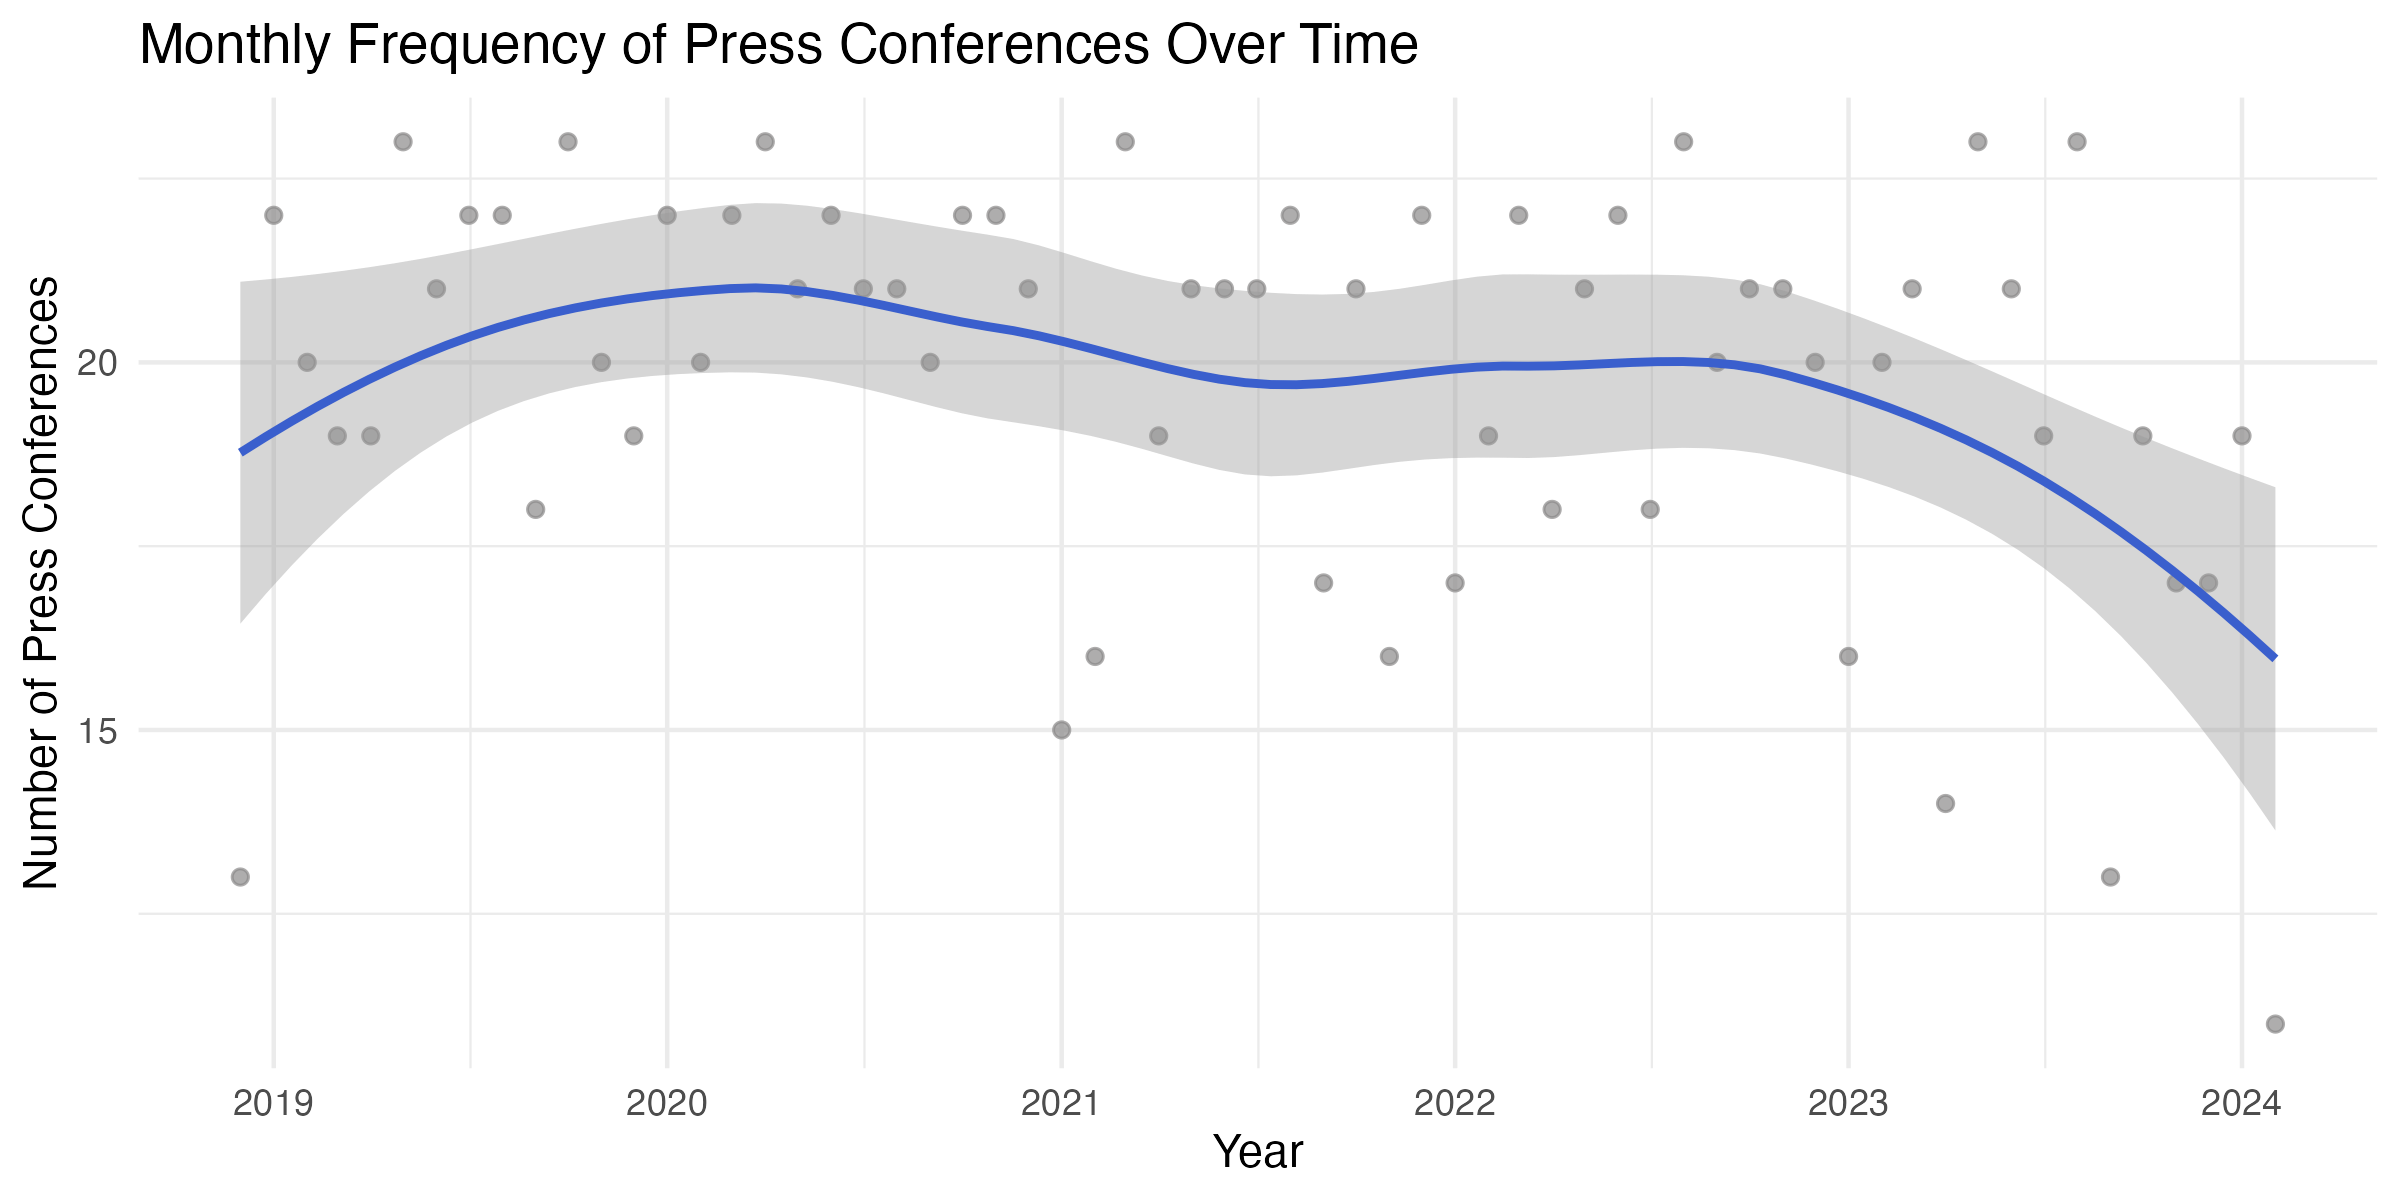
\includegraphics[width=\textwidth]{/Users/sarabcidf/Desktop/ASDS/Dissertation/AMLO/Analysis/conf_freq_time.png}
\end{figure}

\vspace*{\fill}

\newpage
\vspace*{\fill}

\begin{figure}[H]
	\centering
	\caption{\label{}}
	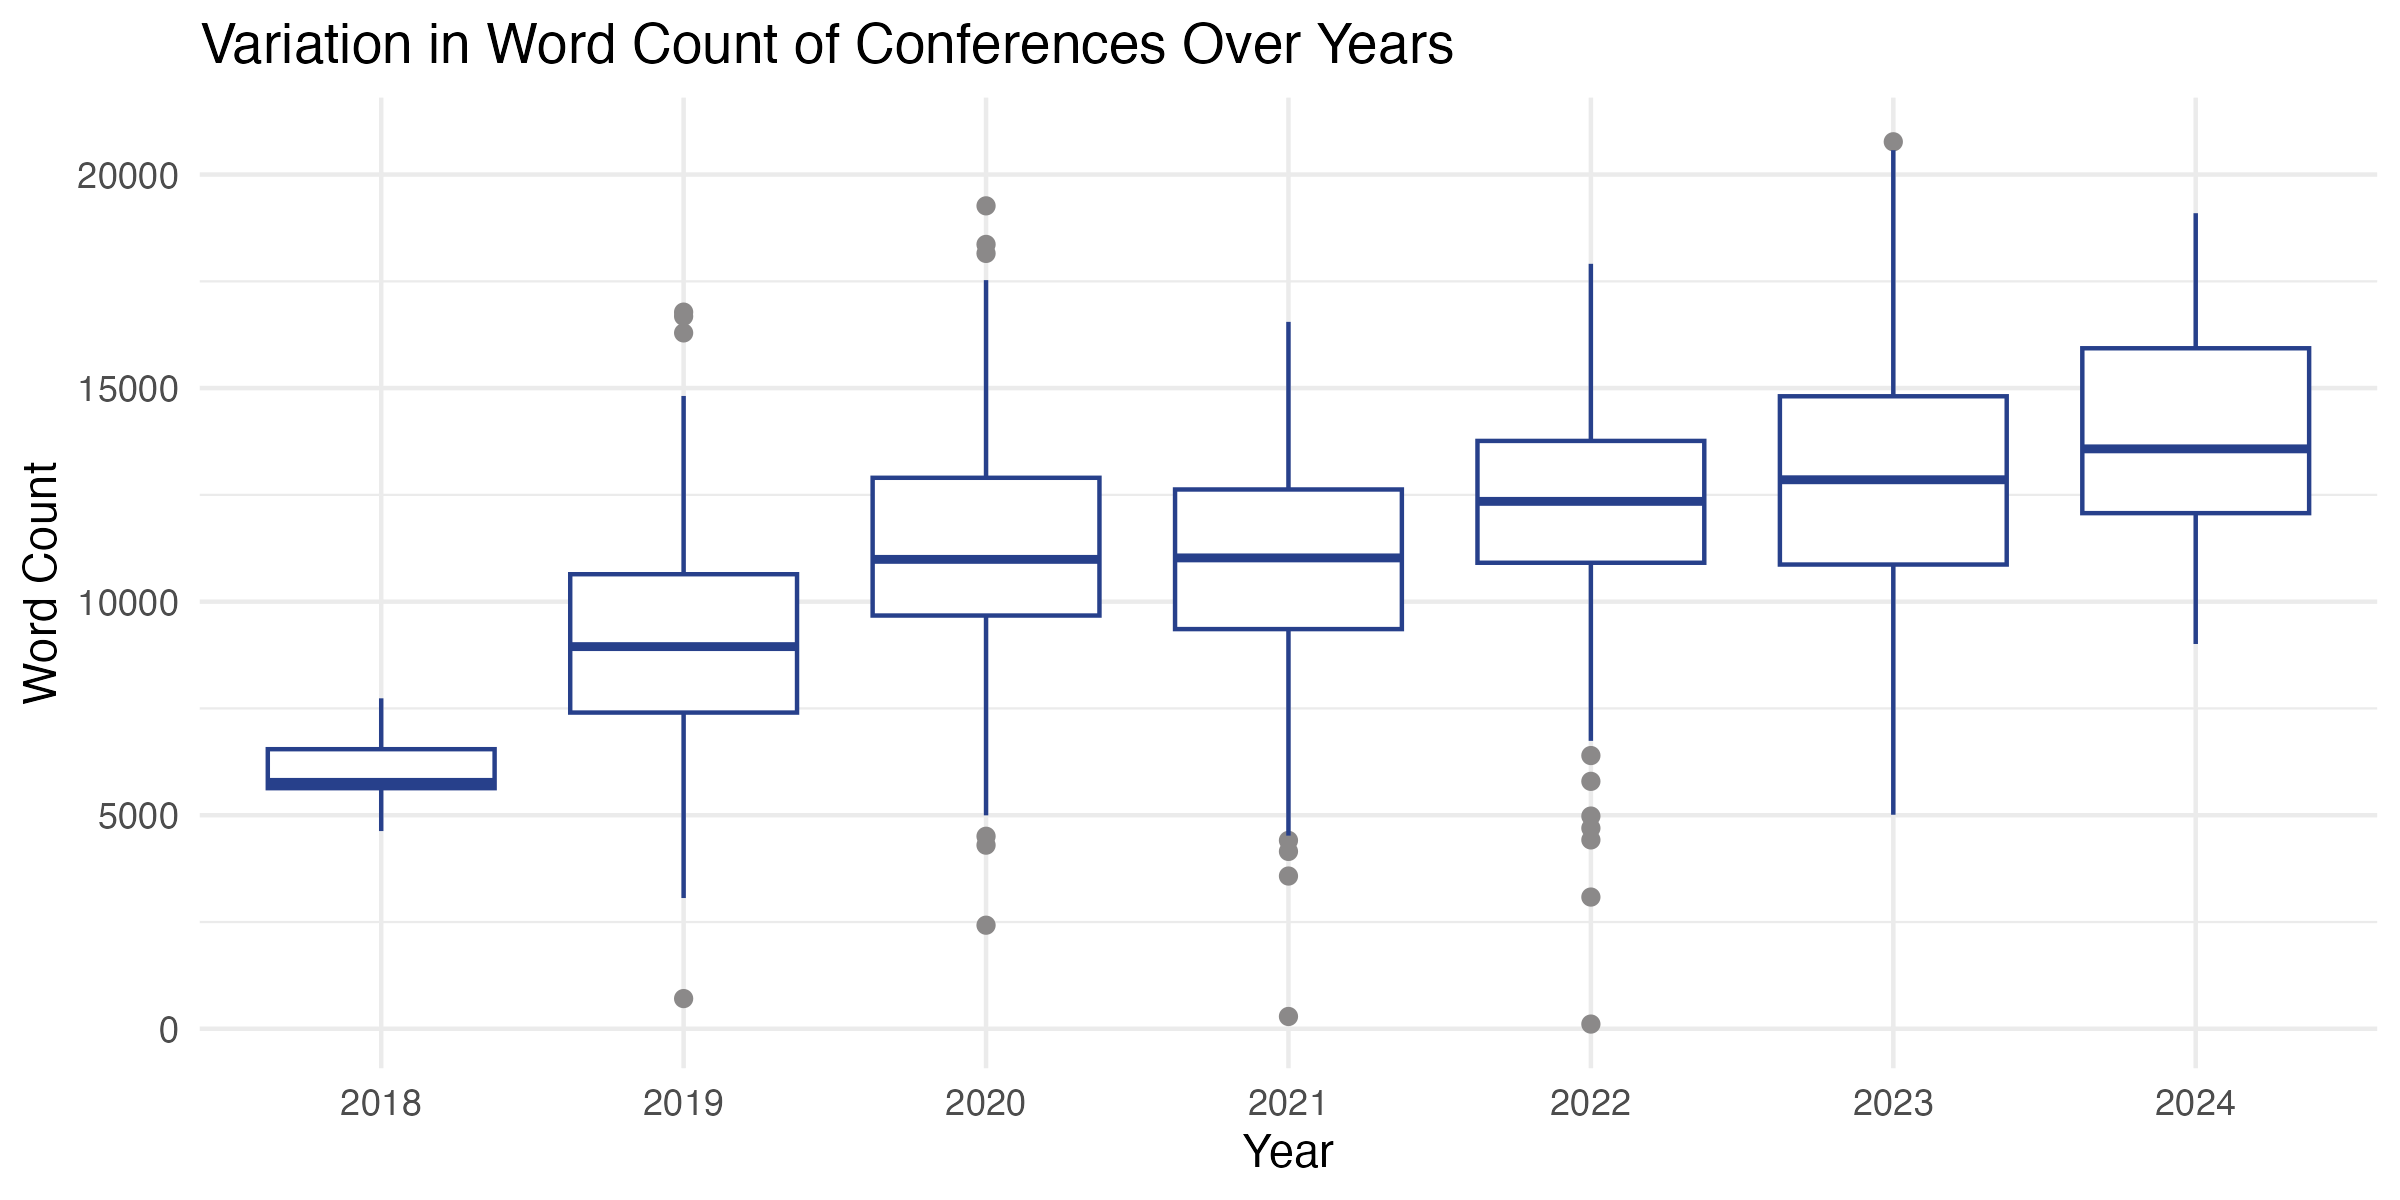
\includegraphics[width=\textwidth]{/Users/sarabcidf/Desktop/ASDS/Dissertation/AMLO/Analysis/var_words_time.png}
\end{figure}

\begin{figure}[H]
	\centering
	\caption{\label{}}
	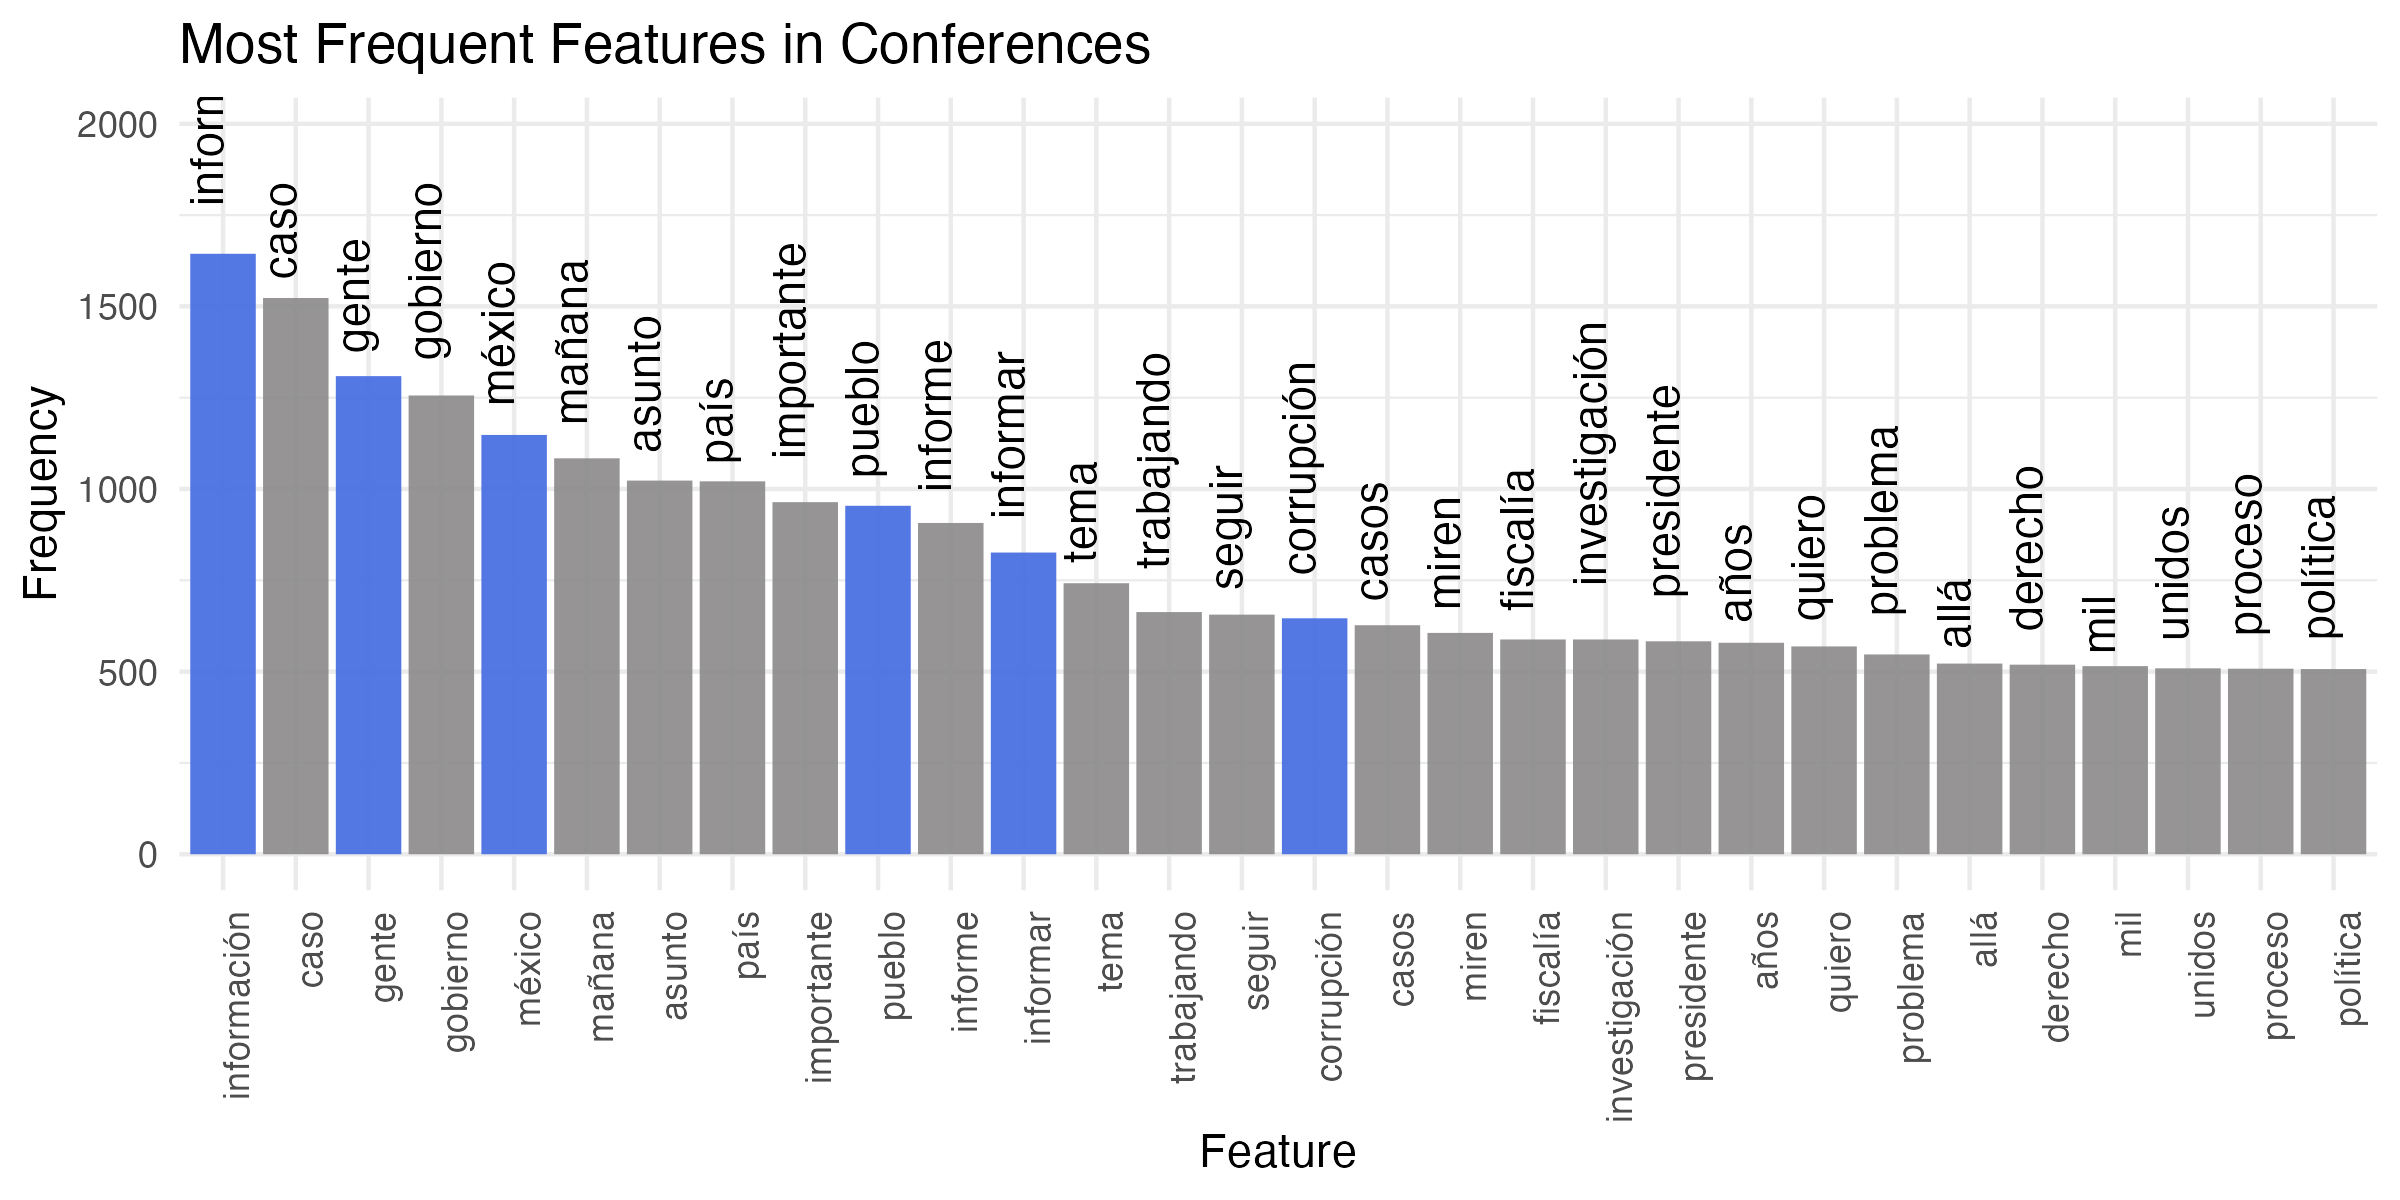
\includegraphics[width=\textwidth]{/Users/sarabcidf/Desktop/ASDS/Dissertation/AMLO/Analysis/TopWords.png}
\end{figure}

\vspace*{\fill}

\newpage
\vspace{.5cm}
\noindent\textbf{Net Sentiment Analysis}
\vspace{.5cm}

Sentiment analysis was performed using translations of the AFINN and NRC sentiment dictionaries. Figure 9 below shows that according to both measures, the sentiment in AMLO's speech has become more positive overt time. NRC detects a larger change, although the average net sentiment remains within close bounds of scores of 3 to 14 points. 

\begin{figure}[H]
	\centering
	\caption{\label{}}
	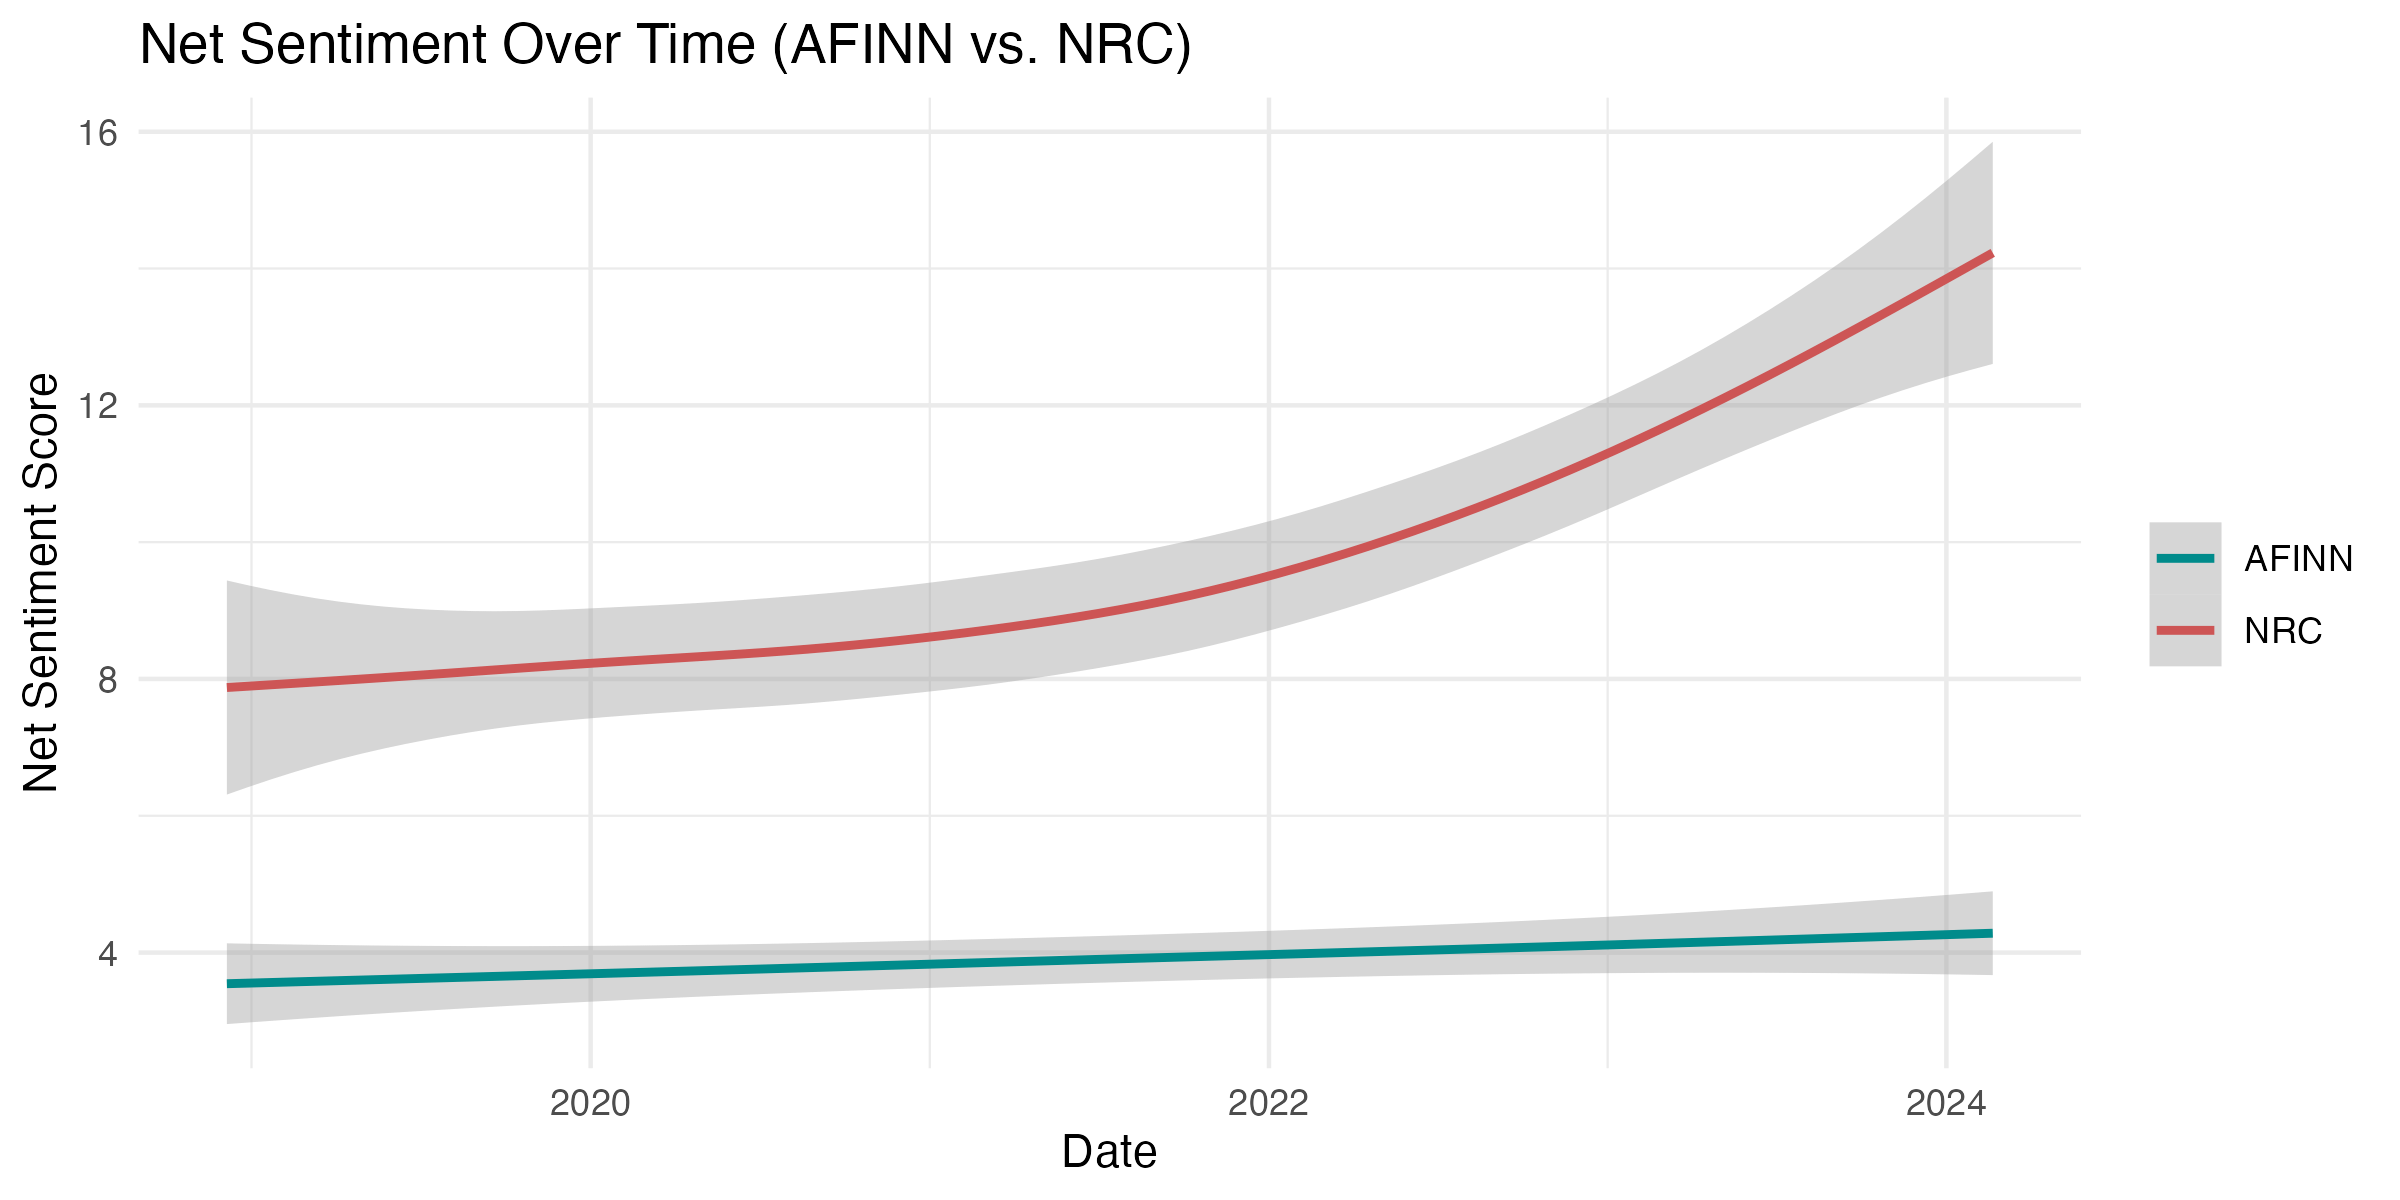
\includegraphics[width=\textwidth]{/Users/sarabcidf/Desktop/ASDS/Dissertation/AMLO/Analysis/senttime.png}
\end{figure}

\noindent\textbf{Populist Dictionary}
\vspace{.5cm}

The table below illustrates the populist dictionary that was applied in this study, in its four versions, and including the English and Spanish versions of words. When some word in Spanish lacks a direct or meaningful translation, this is explained. Also, when several words can express the same (like the plural or individual version of the same thing), both words were included. For instance, both masculine and feminine subjects can be undemocratic in Spanish, so both the male and female version are included, as shown in the first row of the table. 

\setstretch{0.9}	
\begin{longtable}{|p{3cm}|p{4cm}|p{4cm}|}
	\hline
	\textbf{\small Category} & \textbf{\small English} & \textbf{\small Spanish} \\
	\hline
	\textbf{\small Anti-elitism} & \small Original (Roodujn \& Pauwels) & \small undemocratic / antidemocrático/a \\
	& \small caste & \small casta \\
	& \small consensus & \small consenso \\
	& \small corrupt & \small corrupto(s) \\
	& \small dishonest & \small deshonesto(s) \\
	& \small elite(s) & \small élite(s) \\
	& \small establishment & \small poder\_establecido \\
	& \small deceit & \small engaño \\
	& \small lie(s) & \small mentir / mentira(s) \\
	& \small propaganda & \small propaganda \\
	& \small scandal(s) & \small escándalo(s) \\
	& \small betray / betrayed / betrayal & \small traición / traicionar / traicionado(s) \\
	& \small shame & \small vergüenza \\
	& \small truth & \small verdad \\
	\textbf{\small Additional terms (Mexico-specific)} & \small mafia in power; used to refer to the establishment & \small mafia\_poder \\
	& \small derogatory term for rich or high-class & \small fifí(s) \\
	& \small conservative(s) & \small conservador(es) \\
	& \small neoliberal(ism) & \small neoliberal(lismo) \\
	& \small oligarchy & \small oligarquía \\
	& \small opposition & \small oposición / opositores \\
	& \small used to refer to the PRI and the PAN; the largest political parties in Mexico aside from MORENA & \small prian \\
	\textbf{\small People-centrism} & \small Additional people-centric component by Boussalis \& Decadri & \small citizen(s) / ciudadano(s) \\
	& \small consumer & \small consumidor(es) \\
	& \small taxpayer & \small contribuyente(s) \\
	& \small voter & \small elector(es) \\
	& \small people & \small gente / pueblo \\
	\textbf{\small Additional terms (Mexico-specific)} & \small poor / poor\_first & \small pobre(s) / primero\_pobres \\
	\hline
\end{longtable}

\noindent\textbf{Readability and Lexical Diversity}
\vspace{.5cm}

Finally, Figures 10 and 11 below show the results of analyzing AMLO's readability and lexical diversity. First, AMLO scores between 0 and 30 points in the Flesch-Kincaid scale over time, with a downward trend. This range of scores corresponds to a very difficult reading level. Moreover, the downward trend over time suggests that the complexity of AMLO's discourse has been increasing. These results most likely speak to the adequacy of the Flesch-Kincaid measure of readability for Spanish texts, as such high readability scores are far from what is expected. The computation of a more adequate measure of readability for Spanish, such as the Hernández-Huerta measure was beyond the reach of this study, but the analysis of AMLO's language against a more suitable measure would make a productive future endeavor. 

As for lexical diversity, AMLO scores around 0.85, which suggests a high variety of vocabulary. There is also a slightly declining trend overtime that suggests a repetition of language or a narrowing of vocabulary. This result is also the contrary as it would be expected: AMLO should probably express himself with a simpler vocabulary, following the hypothesis about populist language. However, according to this measure, AMLO seems to be far from lacking lexical diversity. Unlike with readability, this could be possible, as AMLO's vocabulary could be both simple and diverse at the same time, which is a relevant finding. 

\newpage
\vspace*{\fill}
\begin{figure}[H]
	\centering
	\caption{\label{}}
	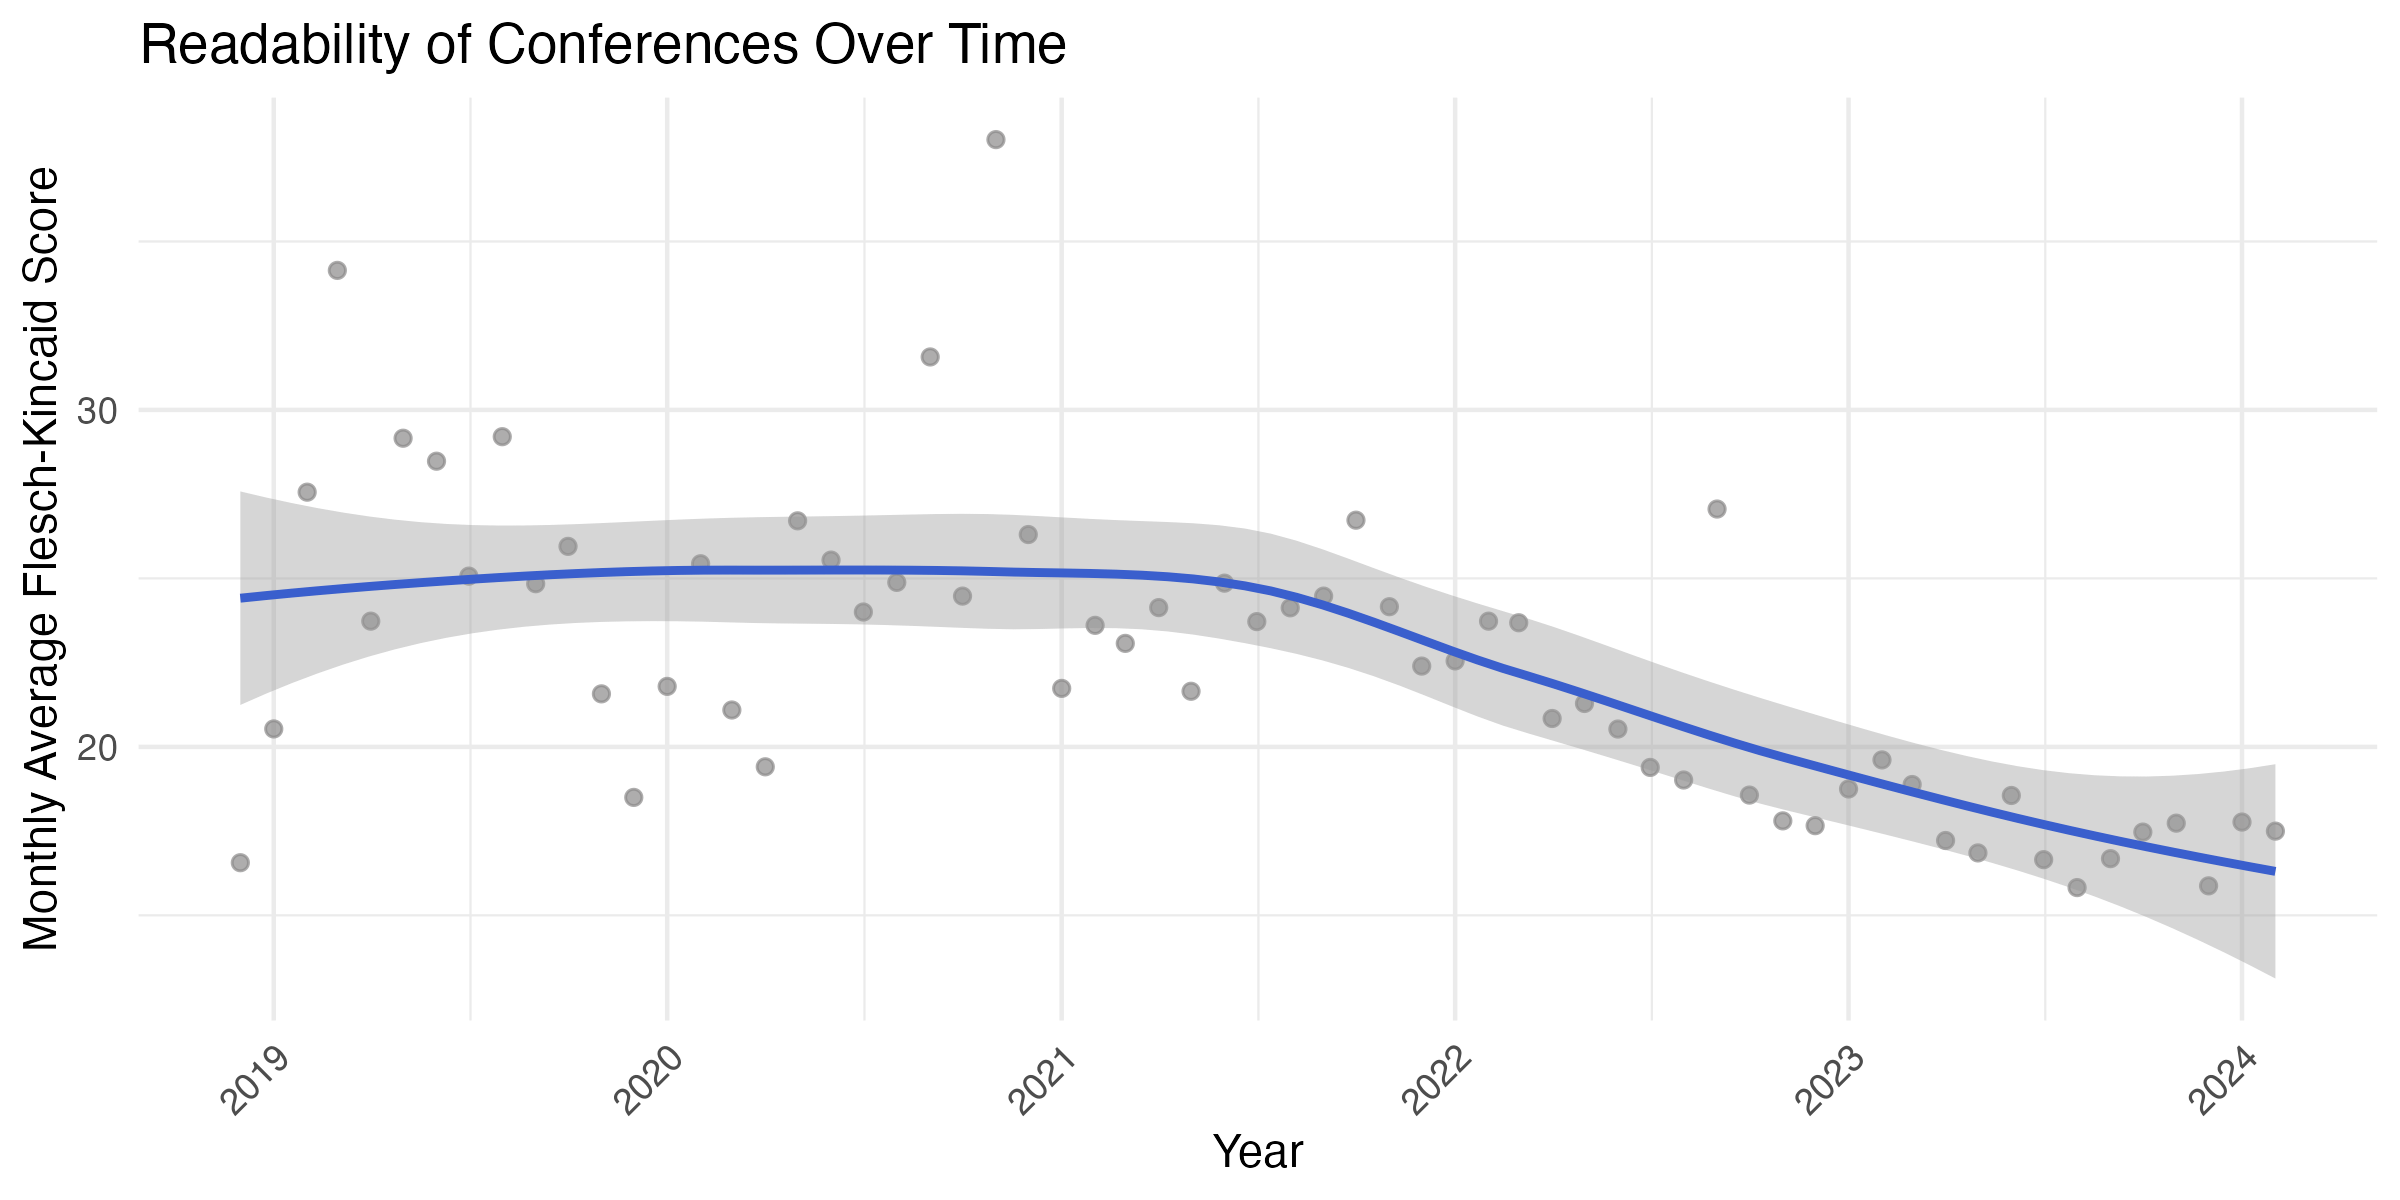
\includegraphics[width=\textwidth]{/Users/sarabcidf/Desktop/ASDS/Dissertation/AMLO/Analysis/readability.png}
\end{figure}

\begin{figure}[H]
	\centering
	\caption{\label{}}
	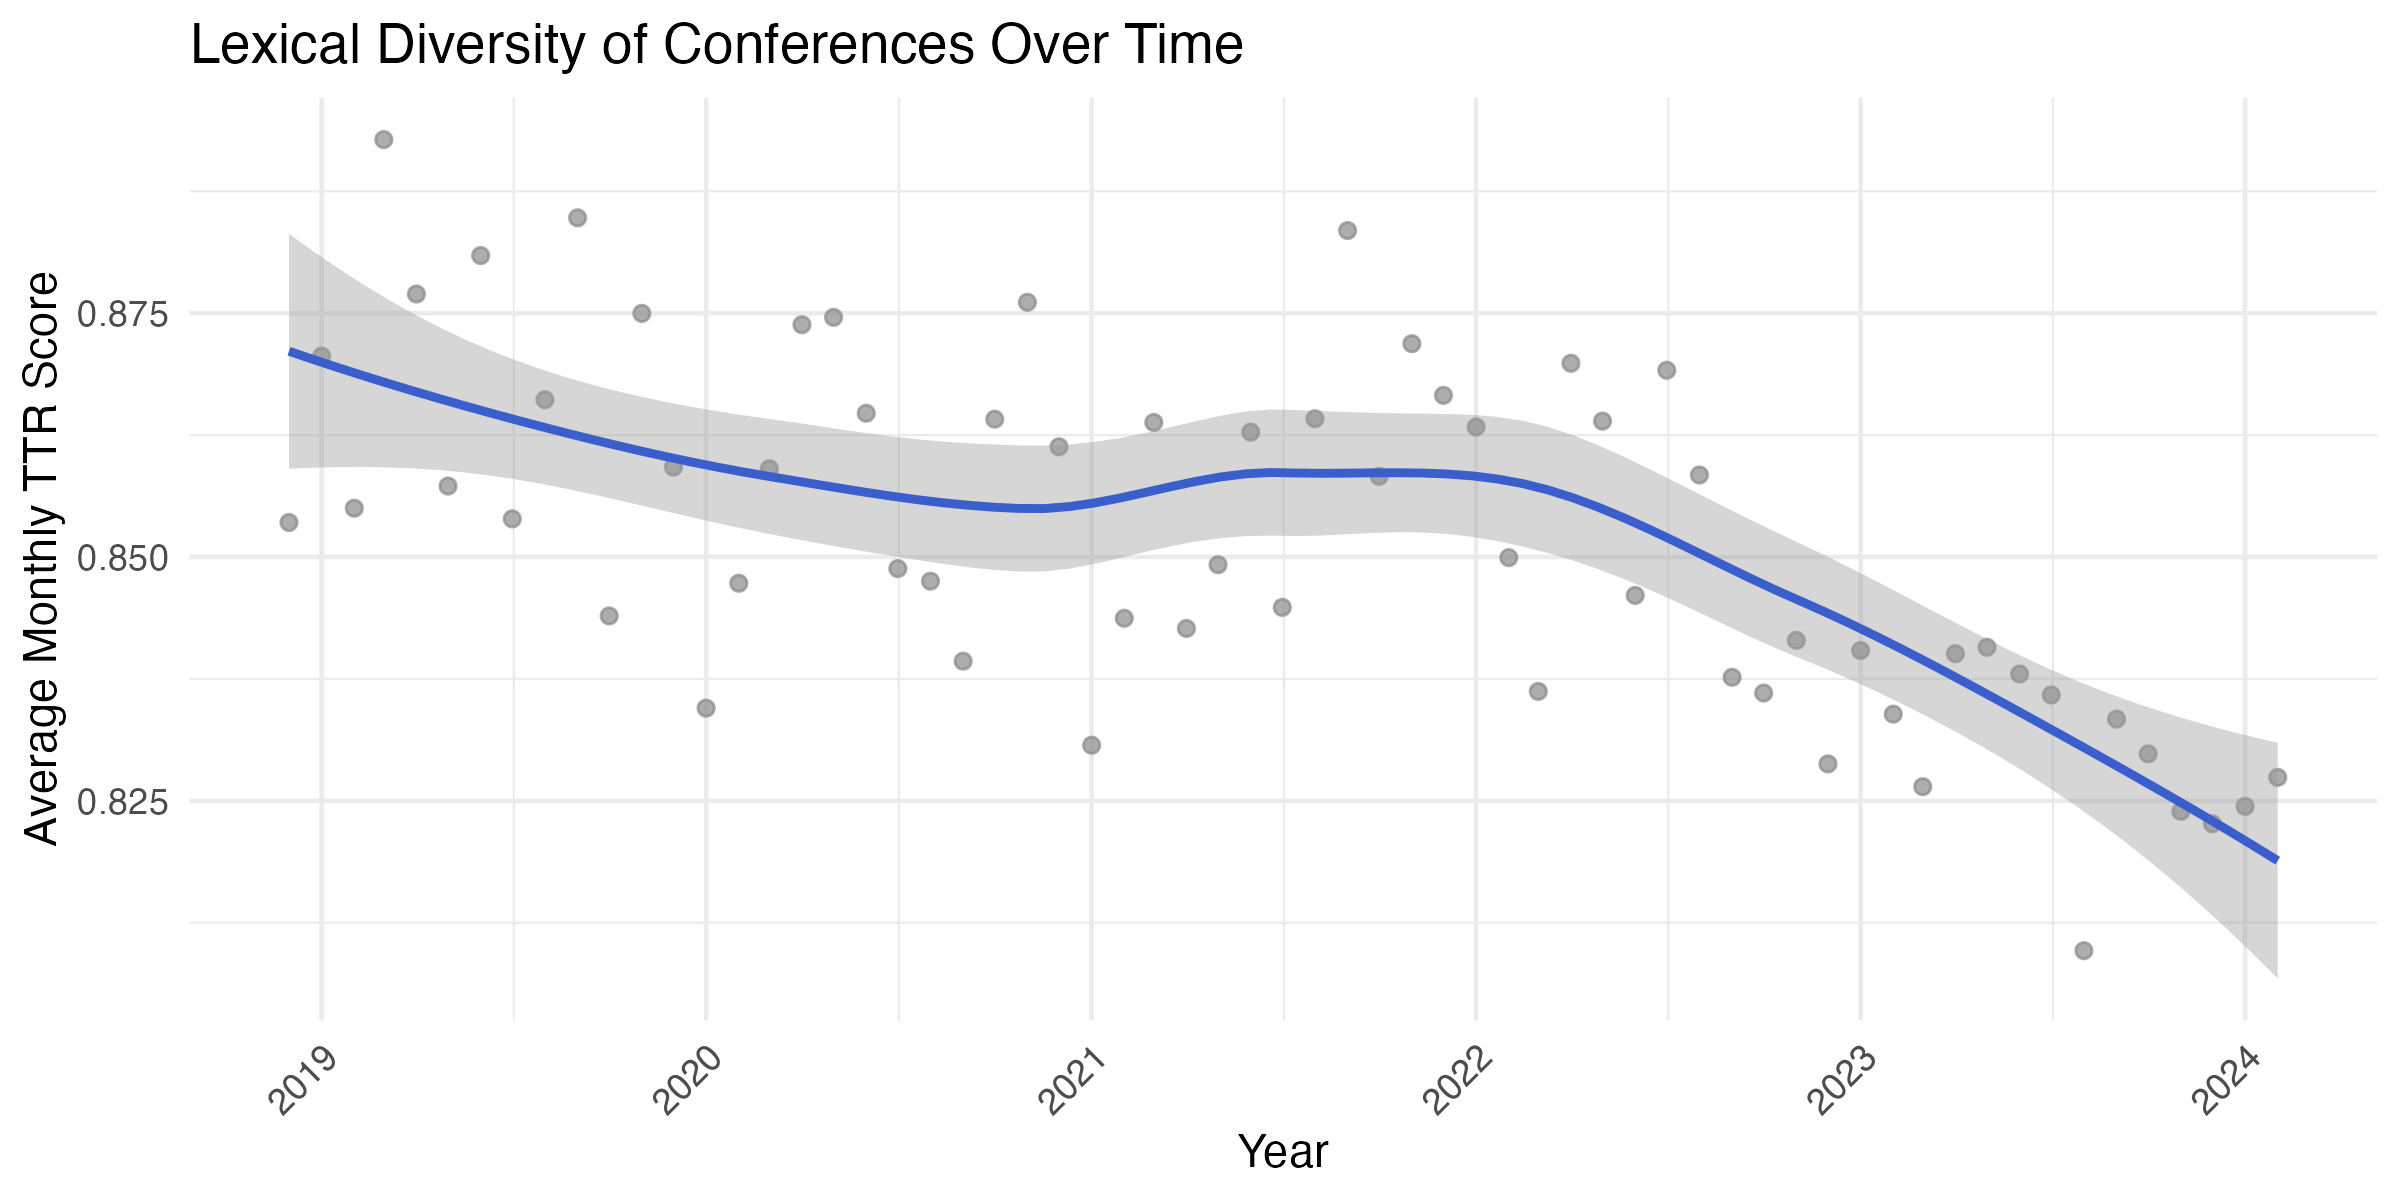
\includegraphics[width=\textwidth]{/Users/sarabcidf/Desktop/ASDS/Dissertation/AMLO/Analysis/ldiversity.png}
\end{figure}

\vspace*{\fill}

\end{document}
